\documentclass[11pt]{report}
\setcounter{tocdepth}{4}
\setcounter{secnumdepth}{4}
\pagestyle{plain}
\usepackage[spanish]{babel}
\selectlanguage{spanish}
\usepackage[utf8]{inputenc}
\usepackage{listings}
\usepackage{color}
\usepackage[table]{xcolor}
\usepackage{graphicx}
\usepackage{amssymb}


% ------------------- Titulo y  Autor -----------------------------
\title{Samplers: Framework para construir aplicaciones Android para recolectar muestras en proyectos de Ciencia Ciudadana}
\author{Laura Lus y Javier Ramírez}

\begin{document}

\maketitle

\begin{abstract}
%Este es un resumen de la tesis muy corto (media carilla). El que lo lee se tiene que quedar con la idea de: 1) en que tema trabajaron, 2) cual es el problema que intentaron resolver, 3) que técnica aplicaron para resolverlo y por qué es novedosa, 4) que descubrieron en el proceso (un adelanto de conclusión). 

La Ciencia Ciudadana involucra al público en proyectos de investigación científica. Las tareas de un voluntario o ciudadano científico pueden ser simples y no necesitar ningún conocimiento especial, o pueden ser más complejas y requerir capacitación previa. Ejemplos de tareas en proyectos de ciencia ciudadana pueden ser contar elementos que aparecen en una fotografía (si aparece un determinado animal o si puede reconocer una galaxia) o bien responder una serie de preguntas para recolectar información sobre un ambiente que el voluntario está observando (podría ser el ecosistema que rodea una laguna o un estuario). 

Hacer partícipes a los ciudadanos de proyectos de investigación científica persigue varios fines, entre de ellos poder realizar investigaciones a gran escala temporal y espacial\cite{bonney2009citizen}, brindar la oportunidad de participar en proyecto reales e interactuar con científicos, o bien perseguir fines educativos. Los proyectos de investigación que incluyen Ciencia Ciudadana pueden clasificarse en acción, conservación, recolección, virtual y educativos \cite{wiggins2011conservation}. 

El presente trabajo se concentra en los proyectos de recolección, que son los que requieren recolectar muestras del medio físico. Más específicamente las que requieren recolectar muestras haciendo uso de dispositivos móviles. 
Samplers es un framework Android para construir aplicaciones que permitan la recolección de muestras utilizando las herramientas que brindan los dispositivos móviles, como puede ser geolocalización o toma de fotografías.

\end{abstract}

\tableofcontents

%Cada capitulo será un archivo .tex el cual estará en su propia carpeta, con sus propias imágenes).
%El comando include hace que el capitulo respectivo se incluya en el documento. No es necesario indicar la extensión 
%del archivo dado que asume que es .tex
%Los números en el nombre de las carpetas son solo para tenerlas ordenadas.

\chapter{Introducción}

\label{introduccion}

%[¿en que tema están trabajando? ] Introduce en contexto en el que están trabajando (p.e., el ámbito en el que se dá el problema). Da definiciones (brevemente) de conceptos que aparecen en el contexto. 

Acá introducción de ciencia ciudadana y samplers \cite{wtf}

\section{ Estructura de la Tesina }
Este trabajo de tesina se organiza de la siguiente manera:
\begin{itemize} 
	\item{Capítulo 1} 
		\begin{description}
		 El propósito de este capítulo es explicar la estructura de esta tesina y dar un resumen de cada capítulo, resaltando sus principlaes objetivos.
		\end{description}


	\item{Capítulo 2} 
		\begin{description} 
		Este capítulo comienza explicando qué es la ciencia ciudadana y cómo es que su popularidad está en aumento. Detalla una clasificación de proyectos de ciencia ciudadana y luego ahonda en uno de los tipos de la clasificación, que son aquellos proyectos donde la inclusión de los científicos ciudadanos se realiza en la recolección de información o muestras. Se describe el método científico ya que los proyectos de investigación que utilizan ciencia ciudadana o cuyo diseño gira en torno a incluir a científicos ciudadanos son proyectos que utilizan las bases de la investigación científica, es decir, son proyectos que utilizan el método científico. A diferencia de los proyectos de investigación donde todos sus participantes son científicos o personas con conocimiento o experticia en el área de estudio, los proyectos de ciencia ciudadana deben tener especial cuidado definiendo los protocolos de recolección de la información para que sus participantes puedan seguirlos. Por último, teniendo en cuenta que los dispositivos móviles están al alcance de muchas personas, presentamos datos de uso de dispositivos móviles y sistemas operativos en el país.
		\end{description}
	
	\item{Capítulo 3} 
		\begin{description} 
		Se introduce el concepto de framework y se describe una clasificación en base a su diseño y tipo de especialización. Luego se describe el estado de tres herramientas que asisten a los investigadores en la creación y la administración de proyectos de recolección que utilizan ciencia ciudadana. Se analizan las ventajas y las desventajas de las herramientas descritas en la sección.
		\end{description}
	
	\item{Capítulo 4} 
		\begin{description} 
		Se describe el sistema operativo para dispositivos móviles Android y se detallan sus principales componentes de aplicación. La Activity, el componente principal de las aplicaciones en Android. Características, ciclo de vida y posibles estados. Relación entre Fragment y Activity. Ciclo de vida y estads del Fragment. Propósito de los Services y tipos soportados. Método de suscripción de eventos del sistema y de otras aplicaciones, BroadcastReceiver. 
		\end{description} 

	\item{Capítulo 5} 
		\begin{description} 
		Samplers, un framework para construir aplicaciones Android para proyectos de recolección que utilizan ciencia ciudadana. Alcance y descripción de la solución propuesta con Samplers. Workflow o protocolo para la recolección de la muestra. Descripción y ejemplo del archivo para configuración de una aplicación. Pasos para la recolección de la muestra: Step y Workflow y su relación con los principales componentes de las aplicaciones Android. Sample, la muestra, resultado de la ejecución del workflow por parte de un científico ciudadano. Envío de muestras por internet y persistencia local para envío manual o cuando tenga disponibilidad.
		\end{description}
		
	\item{Capítulo 7} 
		\begin{description} [Breve explicación de lo que se trata en el capitulo 7]
		\end{description}				
\end{itemize}

\section{ Motivación }

Los proyectos de investigación científica a menudo requieren la realización de gran número de actividades que son difíciles de automatizar como puede ser la clasificación de fotos, anotaciones, observaciones y todo tipo de actividades que en esencia son simples, pero consumen mucho tiempo. Muchas veces estas actividades son sencillas y no se necesita de ninguna preparación académica o escolarizada previa para realizarlas, por ejemplo indicar si en una foto se observa o no un animal. La ciencia ciudadana es una forma de investigación en colaboración que involucra a los ciudadanos resolviendo este tipo de tareas simples en proyectos de investigación científica que buscan resolver problemas del mundo real \cite{wiggins2011conservation}. 

Un científico ciudadano es un voluntario que recoge y/o procesa información como parte de una investigación científica \cite{silvertown2009new}. Para que los voluntarios puedan participar en estos proyectos es necesario brindarles herramientas que los ayuden a contribuir. 
Nuestro interés está enfocado en los proyectos de recolección. Estos proyectos de investigación científica requieren la recopilación de datos del medio físico. Una forma de asistir a estos proyectos es por medio de sistemas informáticos que posibiliten la recolección de datos usando móviles. Un ejemplo de este tipo de proyectos es AppEAR un sistema de ciencia ciudadana para cuidar y aprender de los ambientes acuáticos en Argentina, realizado por Joaquín Cochero, investigador del CONICET en el Instituto Platense de Limnología. El objetivo final de AppEAR es tener un relevamiento completo y detallado de aguas continentales de todo el territorio nacional para conocer los lugares en riesgo en los que urge trabajar. Los voluntarios de este proyecto descargan una aplicación para su dispositivo móvil y toman muestras para el proyecto. La aplicación guía a los usuarios a través de los pasos necesarios para tomar una muestra.

La mayoría de los proyectos de ciencia ciudadana de recolección cuentan con aplicaciones desarrolladas específicamente para cada proyecto, en donde el principal problema a resolver es la secuencia de pasos que conforman el protocolo para la toma de la muestra y la combinación de este protocolo y de las herramientas del dispositivo móvil que se desean utilizar cómo puede ser la cámara, el GPS, el micrófono para grabar un audio. Consideramos que proveer un framework que resuelva esta problemática, la de la aplicación específica de cada proyecto, sería útil para la creciente comunidad de científicos que quieren incluir ciencia ciudadana en sus proyectos.

Este proyecto se enmarca dentro de Cientópolis\cite{cientopolis}, una plataforma para la promoción y el estudio de la Ciencia Ciudadana. Cientópolis se nuclea como un proyecto de investigación desde la Facultad de Informática de la UNLP pero articula su funcionamiento con investigadores de las facultades de Ciencias Astronómicas y Geofísicas, Humanidades y Ciencias de la Educación, Bellas Artes y Ciencias Naturales y Museo.

\section{ Objetivos }		
		
Se propone desarrollar un framework para instanciar aplicaciones móviles Android de ciencia ciudadana. El framework recibirá un archivo con la configuración requerida en formato JSON y generará una aplicación para ejecutarse en un dispositivo Android. En este archivo estará el conjunto de pasos que especifican el protocolo de recolección de muestras. Estos pasos pueden ser:
			\begin{itemize}
				\item captura de una foto, un video, un audio, una ubicación o un recorrido hecho con el dispositivo móvil.
				\item contestar una pregunta con respecto a la muestra. Esta pregunta puede tener una o múltiples respuestas posibles.
				\item introducir anotaciones de texto.
				\item indicar una fecha y hora.
				\item mostrar información de orientación y ayuda para la toma de la muestra.
			\end{itemize}

La aplicación generada servirá para tomar muestras siguiendo el protocolo de recolección especificado y las almacenará y empaquetará en el dispositivo móvil hasta que pueda ser enviada a un servidor web.
		
Se define el formato del archivo de configuración de la aplicación y la información adicional necesaria, como pueden ser credenciales para acceder a los servicios de Google Services o el posicionamiento por GPS.

Instanciar una aplicación básica de ejemplo con el framework en base a un archivo de configuración, que permita tomar algunas muestras y enviarlas a un servidor web que estará configurado para dicho propósito.
			
\chapter{Marco Teórico}
		
	
\section{Introducción a la Ciencia Ciudadana}
    
    Ciencia Ciudadana es un termino que engloba las diferentes maneras en las que los ciudadanos participan en ciencia. Estas actividades pueden ser enviar información desde aplicaciones instaladas en sus dispositivos móviles acerca de especies invasivas, comportamiento de las aves, la cantidad de mariposas presentes al comienzo de la primavera o cualquier otro tema generalmente relacionado a la ecología y la conservación; como así también participar en debates locales de políticas que afectan directamente el ecosistema de una determinada ciudad o zona, como puede ser el fracking, la minería y los pesticidas en la agricultura y de esta manera influir en las políticas locales respecto de cómo regular esas actividades.\cite{envCitizenScience}
    
	Algunos de estos proyectos cuantan con una larga historia de investigación (como el CBC, Christmas Bird Count), otros con gran cantidad de participantes, quienes interactúan a través de foros y aplicaciones web desde la comodidad de sus hogares (como sucede en proyectos como Zooniverse) o bien abarcando grandes extensiones geográficas (como puede ser en The Big Butterfly Count). \cite{shirk2012public} 
		
	Aunque la ciencia ciudadana no es un concepto nuevo, su notoriedad es relativamente reciente. Los científicos ciudadanos o voluntarios ahora participan de proyectos relacionados con el cambio climático, las especies invasivas, la conservación de ecosistemas biológicos, el monitoreo de la calidad del agua y varios tópicos más. Esta popularidad se vio impulsada principalmente por tres factores:

\begin{itemize}
	\item {Disponibilidad Tecnológica}
	La disponibilidad de herramientas tecnológicas que permitan distribuir información acerca de los proyectos y también permitan recolectar la información generada por los voluntarios. De estas herramientas internet es la más representativa, pero la tecnología móvil está jugando un rol fundamental con la popularización de smartphones. \cite{silvertown2009new}
	\item {Reconocimiento del Aporte de los Voluntarios por parte de los Profesionales}
	La participación de voluntarios en un proyecto de investigación aporta diferentes atributos que pueden ser trabajo, poder de cómputo o habilidad \cite{cohn2008citizen}
	\item {Inclusión del Público General en Proyectos Científicos}
	La mejor manera para que el común de la gente entienda y se involucre en proyectos científicos es siendo parte de ellos. \cite{silvertown2009new}
\end{itemize} 

	En ciencias como pueden ser la arqueología, la astronomía o las ciencias naturales la capacidad de observación es a veces es más importante que el equipamiento costoso. Los voluntarios o científicos ciudadanos realizan actividades como parte de un proyecto científico que está especialmente diseñado o bien fue adaptado para que cumplan un rol, ya sea para fines educativos de los mismos voluntarios o para beneficio del proyecto. En los mejores ejemplos, se benefician ambos: los voluntarios y el proyecto.\cite{silvertown2009new}
	Para ello vamos a utilizar la clasificación provista por Wiggins and Crowston para tener un marco de lo que son los proyectos de recolección según esta clasificación, y por qué son los que mejor se relacionan con los proyectos de Ciencia Ciudadana en donde los colaboradores actúan como investigadores de campo recolectando muestras para introducirel tema de la toma y el envío de muestras recolectadas mediante aplicaciones móviles.	

\section{Clasificación de los Proyectos de Ciencia Ciudadana}	

\begin{itemize}
	\item {Acción}
		
		Los proyectos clasificados en esta categoría no son planificados o iniciados por científicos, sino más bien por los ciudadanos, y generalmente requieren un compromiso a lo largo del tiempo en los problemas ambientales locales por lo cual las actividades científicas están orientadas al ambiente físico. 
		
		Estos proyectos solicitan la colaboración de científicos como asesores o consultores, y no como organizadores. Los datos o resultados obtenidos no persiguen un fin académico, sino más bien buscan fundamentar con evidencia para poder tomar acciones sobre alguna situación. 
	\item {Conservación} 
	
	Al igual que los proyectos de Acción, los proyectos de Conservación son fuertemente regionales, y las actividades de los voluntarios están enfocadas mayormente en la recolección de información. La mayoría de los proyectos de investigación tienen contenido o fines educativos. También tienden a ser de alcance regional, como lo reflejan sus desafíos y metas.
	
	Estos proyectos buscan generar información principalmente como fuente para la toma de decisiones relacionadas al manejo de recursos, y también buscan la promoción de la administración y reconocimiento del voluntariado. También prestan especial atención a la generación de información científicamente válida. Son esfuerzos de monitoreo a largo plazo y generalmente no tienen problemas de sustentabilidad, ya que son subvencionadas por fondos públicos o reciben ingresos de agencias que son las que nuclean los proyectos o son las interesadas en sus resultados.
	
	\item {Investigación o Recolección} 
	
	Los proyectos de investigación concentran su atención en investigaciones científicas cuyos objetivos requieren la recolección de información del medio físico. Este tipo de proyectos es el que mejor encaja en la definición de Ciencia Ciudadana. Y aunque los objetivos de educación no son los principales de estos proyectos, forman parte de ellos como material de capacitación o incluyendo estructuras de recolección que alientan el aprendizaje al aire libre. El alcance varía de regional a internacional, y puede lograr participación masiva de hasta decenas de miles de voluntarios y obtener millones de observaciones (de voluntarios) anuales. La mayoría de estos proyectos están enfocados en la investigación biológica, medioambiental o meteorológica, por dar algunos ejemplos. 
	
	Una de las principales preocupaciones de este tipo de proyectos es generar resultados científicamente válidos, ya que son concebidos para generar conocimiento formal y son mayormente organizados por científicos. El cuidadoso diseño del proyecto y de las tareas son los que permiten lograr resultados válidos. Aparte utilizan toda una serie de metodologías que permiten la validación de la información generada. Los voluntarios están dispersos geográficamente y esto es un recurso valioso ya que este tipo de proyectos intenta muchas veces registrar la distribución geográfica de determinadas especies o la ocurrencia de fenómenos naturales. 
	
	\item {Virtual} 
	
	En los proyectos de ciencia ciudadana denominados Virtuales todas las actividades son mediante tecnologías de la información y la comunicación, sin la intervención de elementos del entorno físico.
	
	Los proyectos que cumplen las condiciones para ser clasificados como virtuales provienen de la astronomía, la paleontología y la proteómica, que es una rama de la microbiología que estudia la estructura de las proteínas. Algunos proyectos de psicología podrían clasificar, pero no lo hacen porque los voluntarios colaboran como sujetos de pruebas, y esto no es formalmente considerado como colaboración en la investigación. 
	
	Galaxy Zoo es un ejemplo de proyecto virtual de ciencia ciudadana. Desde hace más de diez años los voluntarios que colaboran con el proyecto clasifican galaxias en fotografías. Responden una serie de preguntas respecto de la foto que están observando, y de esta manera los científicos encargados del proyecto obtienen una primera clasificación, que se construye en base a las observaciones de varios voluntarios de manera independiente. \cite{GalaxyZoo} 
	
	Al igual que en los proyectos de recolección anteriormente mencionados, los proyectos virtuales encuentran dificultades a la hora de conseguir resultados válidos en términos científicos. Estos resultados se obtienen mediante el desarrollo cuidadoso de las actividades. Como la participación es mayormente virtual, poder mantener a los voluntarios comprometidos con el proyecto es un desafío. Por eso muchas veces estos proyectos incluyen técnicas de gamificación, de competencia amigable entre participantes o de valoración de la contribución hecha por el voluntario (feedback).
	 
	\item {Educación} 
	
	Los proyectos de ciencia ciudadana pertenecientes a esta categoría son aquellos cuyo principal objetivo es educar. Los participantes de estos proyectos tienen como objetivo educar, y aportan recursos educativos informales; mientras los proyectos ofrecen material educativo formal. También, las actividades están pensadas para que el participante vaya acumulando conocimientos.
	
	Un ejemplo de este tipo de proyectos es Fossil Finders, que centra la investigación en el análisis de fósiles del Devónico (período de la era Paleozóica) proveyendo de materiales de estudio a estudiantes y profesores de escuelas secundarias. Los estudiantes van a identificar y medir fósiles en muestras de rocas enviadas a sus aulas. Luego ingresarán los datos obtenidos en una base de datos online, y podrán comparar sus datos con los de otras escuelas participantes. Con ello van a tener la oportunidad de involucrarse con métodos de investigación reales y de asistir a los investigadores del Instituto de Investigación Paleontológica a reconstruir el pasado geológico de Nueva York. \cite{FossilFinders}

	La mayoría de estos proyectos proyectos persiguen un fin educativo, el aprendizaje y el desarrollo de habilidades científicas. Por ello incluyen actividades de análisis de datos o muestras, brindando la posibilidad de desarrollar pensamiento crítico. 
	\end{itemize} 
	
	Los proyectos de Ciencia Ciudadana buscan resultados que generalmente caen en tres grandes categorías: resultados que sirven a la investigación; resultados que le sirven a los participantes como pueden ser adquirir nuevas habilidades o conocimientos y/o resultados que tienen que ver con sistemas socio-ecológicos, como es influenciar políticas, construir bases para la toma de decisiones en una comunidad o participar de acciones para la conservación del medio ambiente. \cite{shirk2012public}

\section{Proyectos de Recolección}	 
	En los proyectos de recolección, según la clasificación antes descripta, es en donde Samplers  brindaría su aporte, ya que está pensado para crear aplicaciones Android que sirvan para recolectar muestras en proyectos de Ciencia Ciudadana.
	
	Hay tres puntos en los que se debe enfatizar para que los voluntarios pueden recolectar y enviar información confiable: proveer información clara acerca de los protocolos de recolección, proveer formularios para el ingreso de datos que sean lo más lógicos y simples posibles y por último brindar soporte para que los participantes entiendan cómo seguir los protocolos y cómo enviar la información.\cite{bonney2009citizen}

\begin{itemize}
	\item {Protocolos}	
			Los datos que se obtienen en proyectos de Ciencia Ciudadana son recolectados mediante protocolos que especifican dónde, cuándo y cómo esos datos deben ser recolectados. Los protocolos deben definir un diseño formal o un plan de acción que permita combinar las muestras que fueron tomadas por múltiples participantes en diferentes ubicaciones para su posterior análisis. Los protocolos utilizados en proyectos de ciencia ciudadana deben ser fáciles de ejecutar, deben poder ser explicados de manera simple y directa, y deben ser desafiantes para los voluntarios.\cite{bonney2009citizen}
		Como se explica más adelante, la implementación del protocolo de recolección de muestras es el workflow de Samplers.
		
	\item {Formularios de ingreso de Datos}	
			En conjunto con un protocolo de recolección bien diseñado están los formularios de ingreso de datos. Los formularios en los que los usuarios ingresan sus observaciones deben ser fáciles de entender y completar. En cada paso de su wokflow, Samplers provee formularios de ingreso de datos que pueden ser preguntas de respuesta simple o compuesta (como componentes radio o checkbox), permite sacar fotografías o informar una ubicación entre otras funcionalidad provistas. 
			Es recomendable definir límites en el rango de datos que los formularios recogen para simplificar su posterior análisis. Por ejemplo, si la respuesta esperada a la pregunta 'Cuántos árboles cuenta en una cuadra' debería ser un número entre cero y 15 una respuesta como 150 podría indicar un error de tipeo. Entonces, es aconsejable pedirle al usuario que reporta que chequee si la información ingresada es correcta. De esta manera, los usuarios pueden revisar sus respuestas cvuando están fuera de los rangos establecidos. Aun así, suponiendo que el usuario indique un respuesta de esas características, es decir, una respuesta que se salga de los límites esperados; ese formulario debería guardarse con alguna marca que permita identificarlo para que los responsables del proyecto puedan analizarlo con más detalle y ver si se debe a un cambio en el entorno que está siendo observado o si es realmente un error de ingreso de datos del usuario.
			
	\item {Material Educativo}
		Los participantes deben ser provistos de material educativo para entender y seguir de manera satisfactoria los protocolos del proyecto. El material educativo puede incluir guías de identificación, posters, manuales, videos, podcasts, listas de correo y FAQ para que los participantes puedan consultar e incluso participar en foros y discusiones acerca del relevamiento que están haciendo o de cómo se espera que completen los formularios provistos. 
		Samplers ofrece ayuda en cada formulario o ventana de ingreso de datos que puede ser configurada para brindar información acerca de cómo se espera que el voluntario la complete.
		
\end{itemize} 

	
\section{Ciencia Ciudadana y Dispositivos Móviles}	

	Los proyectos de ciencia ciudadana para ampliar su alcance a múltiples lugares, lograr expandir su permanencia en el tiempo y llegar a diferentes escalas sociales necesitan adoptar las nuevas tecnologías. De esta manera, mediante la utilización de tecnologías móviles como smartphones y tablets, tienen la posibilidad de involucrar audiencias más amplias, motivar voluntarios, mejorar la recolección de información y controlar su calidad.\cite{newman2012future}
	(Estadísticas de distribución de móviles) 
	Los dispositivos móviles tienen integrados servicios de captura de imagen (cámaras) y de posicionamiento (GPS) que mejoran la frecuencia y la calidad de la información relevada.\cite{newman2012future}
	
	La proliferación de tecnologías móviles está enriqueciendo los ambientes urbanos en lo relacionado a sensing, proveyendo herramientas para recolectar datos y creando oportunidades para que el común de la gente pueda involucrarse en actividades científicas. En resumen, los dispositivos móviles son ideales para la recolección espontánea de información por el común de la gente. Ahora bien, detrás de su facilidad de uso y de su masividad hay una complejidad técnica y de infraestructura a la hora de desarrollar aplicaciones, que pueden significar una inversión de tiempo, dinero o ambas y pueden limitar el acceso de pequeñas organizaciones o proyectos a este tipo de desarrollos. \citep{kim2013sensr}
	
	



\chapter{Características de los Proyectos de Recolección}

\section{Proyectos de Recolección}

	
%Los proyectos de recolección generalmente tienen algunas complejidades particulares. Se necesita mucha gente para tomar las muestras, cubren grandes extensiones de territorio. Los voluntarios son imprescindibles en estos proyectos, pero también la capacitación previa o conocimiento en el área aportan. La toma de muestras sigue determinado conjunto de pasos cuyo orden debe respetarse para que la muestra sea considerada una muestra. %

\subsection{El Método Científico}
No podemos hablar mucho acá, sino más que nada dar una introducción al método científico, que es el que determina por qué una muestra es una muestra, explicar un poco cómo sería el protocolo de la toma de muestras de campo y eso. Esto podemos consultarlo, para ver de donde sacara bibliografía.

\subsection{Toma de Muestras}

	El artículo Citizen Science: Can volunteers do real research? describe el caso de un voluntario que colabora \textit{con un proyecto de ciencia ciudadana en el Appalachian Trail}. Luego de caminar varios kilómetros, se detiene en un lugar predeterminado y saca su GPS para estar seguro de que es el lugar correcto. Se aparta del sendero peatonal y busca un sendero menos transitado en el bosque más denso. Encuentra un camino lleno de huellas de ciervo y excremento que le indica que es el camino que está buscando.
	
	Este voluntario preside el Natural Bridge Appalachian Trail en Lynchburg, y camina de un lado a otro buscando una cámara digital que dejó en un árbol un mes atrás. Luego de buscar durante varios minutos la encuentra. Apaga la cámara, reemplaza la tarjeta de memoria y las pilas. Vuelve al sendero con huellas de animales, lo recorre dos tercios de milla y lo vuelve a dejar en otro árbol cuidando que el objetivo apunte al sendero. Luego se pone en la mira de la cámara y se mueve hasta escuchar el obturador activado por el sensor de movimiento. 
	
	De esta manera el y otros cientos colaboran con un proyecto de censado de mamíferos del Appalachian Trail desde el sur de Virginia hasta Pennsylvania, y manejan equipamiento, recogen información y anotan observaciones como uno de los varios proyectos que manejan en conjunto agencias gubernamentales, universidades, grupos de conservación ecológica y científicos para supervisar las tendencias ambientales en las cerca de 2175 millas del Appalachian Trail. Tanto el censo de mamíferos como el Appalachian Trail MEGA Transect dependen de voluntarios. Los científicos ciudadanos ayudan a supervisar animales salvajes, plantas u otros objetivos medioambientales y no reciben un pago por su colaboración e incluso a veces no son científicos profesionales. Son aficionados que colaboran con estos proyectos porque disfrutan de estar afuera o porque están comprometidos con los problemas ecológicos y quieren hacer algo al respecto. Generalmente no analizan la información o escriben artículos científicos, pero son esenciales para recolectar la información en la que luego se basan los estudios. 
	
	La Ciencia Ciudadana no es nueva. Lo que es nuevo es la cantidad de voluntarios que se enlistan para colaborar en los estudios, y la amplitud de la información que se les pide recoger. Los investigadores a menudo les piden a los colaboradores que utilicen equipamiento y técnicas sofisticadas para monitorear la calidad del aire y el agua; que documenten el crecimiento, la floración y la muerte de las plantas o que observen cuando las aves y otros animales migran atravesando un área o de qué manera se comportan mientras están en la misma. 
	
%En esta sección podemos ampliar el tema de las características de los proyectos de recolección. Hablar de CBC que abarca una parte muy grande de América del Norte, podemos hablar del proyecto de investigación por el cual AppEAr existe, que es el relevamiento de estuarios en Argentina. Podemos hablar de la app africana para relevar determinadas cosas que hay en terrenos súper inaccesibles, esta app es súper interesante porque es sólo pictográfica, lo que la vuelve amigable para mucha de la gente que no sabe leer ni escribir. %

\subsection{Protocolos de Recolección de Muestras}

	Los protocolos para recolección de muestras en proyectos que incluyen a científicos ciudadanos deben ser simples. Es más sencillo pedir que se identifique, documente o cuente 5 o 10 especies diferentes de plantas que sean fácilmente reconocibles y que serviría para indicar que la especie está presente en el área, en vez de pedir que se identifiquen todas las especies presentes en un área determinada. Una manera de ayudar a los voluntarios es darle libros con guías o material impreso que los ayude.
	
	Como hacemos referencia en el marco teórico, en los primeros estudios la información recolectada por los científicos ciudadanos era imprecisa como para ser utilizada. El principal problema es que la información generada por los voluntarios a veces representan valores en un rango en vez de números específicos, lo que dificulta la detección de cambios en los valores o fundamentar conclusiones. Ahora, los científicos ciudadanos son entrenados para leer instrumentos y recolectar números específicos. Esto debe seguir siendo compatible con protocolos de recolección simples. De esta manera se evitaría caer en el error de solicitarle a los voluntarios la recolección de información muy compleja o detallada. Pero algunas veces se puede solicitar este tipo de complejidad o precisión en la recolección de información. Pero esto no siempre es así. Muchos de los voluntarios que participan en los estudios tienen algún tipo de conocimiento acerca del método científico. De todas maneras debe esperarse información de calidad variada. En esos casos los científicos que dirigen los proyectos deben estar preparados para escrutar cuidadosamente la información obtenida y deben estar dispuestos a descartar información sospechosa o poco confiable.\cite{cohn2008citizen} 
		
\subsection{Diseño de Proyectos de Ciencia Ciudadana}

	El diseño y la implementación de cada proyecto requiere que se tomen decisiones acerca de los intereses de qué público se podría y  debería ser tenido en cuenta a la hora de perseguir intereses, y cómo los objetivos finales, o resultados esperados son definidos. En algunos campos donde puede participar la ciencia ciudadana, las decisiones de diseño son guiadas por teorías de participación, experiencia, o democracia.
	
	A la hora de diseñar un proyecto, una de las primeras preguntas que hay que responder es 'a los intereses de quién/es sirve?'. De esta manera van a quedar un conjunto de opciones resultantes a tomar para implementarlo. Es la negociación entre los intereses científicos y los intereses públicos lo que puede influenciar un rango de resultados potenciales. Public Participation in Scientific Research \citep{shirk2012public} propone un framework para diseñar proyectos de ciencia ciudadana. Los elementos de este framework  son entradas, actividades, salidas, resultados e impacto. 
	
\begin{itemize}
	\item {Entradas}
		Los proyectos de ciencia ciudadana son, por la forma de definirse, un esfuerzo colaborativo, y es por ello que su diseño debe permitir entradas de múltiples constituyentes. Es decir, sus participantes tiene múltiples capacidades y múltiples maneras de brindar su colaboración. Por dar un ejemplo, hay varias maneras de describir una misma imagen. Algunas pueden ser más extensas y detalladas y otras descripciones pueden serlo menos. Estas entradas son los intereses (las esperanzas, deseos, objetivos y expectativas) tanto del público como de la comunidad científica en conjunto a la hora de determinar el objetivo de un proyecto. Podría haber más intereses, pero se considerarán estos dos, las entradas del framework.
		
		Para los voluntarios, sus intereses pueden ser contribuir a generar conocimiento científico, recolectar y diseminar información con respecto a peligros medioambientales, afectar la administración de recursos, proteger [livelihoods], o para satisfacer necesidades que tienen que ver con su identidad personal u objetivos de aprendizaje. Y aunque sería fácil asumir que los intereses de los científicos son principalmente conseguir resultados científicos, bien podrían estar interesados en afectar la educación, la conservación, en manejar la información surgida de sus propias observaciones,o cualquiera de los intereses atribuidos a los voluntarios. Además, estos intereses no son homogéneos incluso dentro del mismo grupo de investigadores o comunidad científica. Y, para tener en cuenta, la línea que divide a los individuos considerados 'científicos' de los que son 'el público' suele no estar bien definida.
		
\end{itemize}	


\section{Ciencia Ciudadana y Tecnología}

	Los teléfonos celulares son dispositivos que están presentes en casi todos los ámbitos y su capacidad de capturar, clasificar y transmitir imágenes, acústica, ubicación y otra información de manera autónoma o interactiva está en crecimiento.
Planteando la arquitectura adecuada, pueden actuar como una red de sensores e instrumentos de recolección de información de localización. 
Esta forma de red de sensores distribuidos puede tener aplicaciones científicas, industriales y militares. Se sabe menos acerca de su función y utilidad en la esfera pública, es decir cuando los que los operan y poseen son usuarios regulares.   Estos sensores en vez de estar en manos de un coordinador central, están siempre bajo el control de sus dueños.

	Solicitar que los dispositivos móviles que ya están [deployados] en el campo, que armen redes de sensores de manera interactiva, participativa y que le permitan a los usuarios del público general y a los profesionales reunir, analizar y compartir información regional. Los micrófonos y cámaras que están presentes en el [handset] del dispositivo pueden registrar información del entorno, mientras se siguen integrando otros sensores de manera inalámbrica. La localización brindada por las antenas de telefonía, el GPS y otras tecnologías proveen información de ubicación y [time-synchronization]. [Las radios wireless] La conexión y el procesamiento que brinda el dispositivo permiten la interacción con la información procesada tanto de manera local como en servidores remotos. 
	
	Los legisladores (creadores de políticas públicas), investigadores y la comunidad utilizan información para comprender y convencer; a mejor calidad de información se consigue una mejor comprensión y políticas significativas. Un ejemplo de ello es la preocupación ciudadana de la ciudad de Los Angeles, cuyos ciudadanos pudieron establecer una relación entre la contaminación del aire y la salud pública. El área contaminación del aire y salud pública es ampliamente estudiada en todo el país utilizando métodos de recolección de datos de manera top-down y bottom-up, y se estima que una red de recolección de datos aportaría una contribución valiosa. El artículo "Elemental Carbon and PM2.5 Levels in an Urban Community Heavily Impacted by Truck Traffic" documenta un estudio hecho de manera conjunta entre la universidad y la comunidad acerca de circulación desproporcionada de tránsito pesado y las tasas de asma registradas. De esta manera, los investigadores de la universidad local llevaron adelante el monitoreo de partículas con equipamiento especializado y con la colaboración de la comunidad para documentar el tráfico comercial de camiones, y eventualmente relacionar la densidad del tráfico con los niveles de partículas saturados de diesel y evidenciar el uso ilegal de rutas no comerciales; información que pueden influir sobre políticas públicas y de salud.
	
	Una arquitectura que permita el participatory sensing puede mejorar y sistematizar la metodología existente incrementando la cantidad, calidad y credibilidad de la información reunida por la comunidad. Implementando protocolos de recolección de información adaptativos basados en estadísticas locales o globales, el participatory sensing facilitaría datos confiables mediante geolocalización, o habilitando la subida automática de información desde equipamiento especializado que todavía no esté conectado a una red. En proyectos con diseño profesional de recolección de datos, se puede incrementar la información recabada distribuyendo observaciones previas hechas con aplicaciones que estén en distribuidas entre los participantes; por ejemplo, conteos previos de cantidad de camionetas en el tránsito del lugar.
	
	Entonces el protocolo adaptado de recolección de información, la ayuda brindada desde la aplicación, la geolocalización y la hora de la toma de la muestra incrementa la confiabilidad de la información generada. Con esta información también se podría detectar en qué lugares o momentos falta recolectar información, y podría pedirle a los participantes que toma la muestra, de ser posible, a una hora determinada o en un lugar en particular. La utilización de auriculares y micrófonos (handset) se abren las posibilidades de capturar información relativa a la exposición individual y la actividad. Además de la recolección de datos interactiva, muestras de audio tomadas en forma periódica del medio que rodea al usuario pueden ser analizadas para detectar si el dispositivo está en medio de un embotellamiento, uno de los motivos principales de la exposición a partículas de diesel. Los dispositivos móviles pueden ser utilizados para detectar patrones de actividad de las personas para establecer la correlación entre los datos recolectados por agencias gubernamentales y obras sociales (healthcare providers); dicha información podría ayudar a los médicos a analizar patrones de exposición a partículas de pacientes, y también en el análisis de actividades y exposición de comunidades. \cite{burke2006participatory}
	
	
	[Pasa a explicar privacidad a la hora de compartir información]
\chapter{Frameworks para proyectos de ciencia ciudadana}

\section{Frameworks}

	Framework podría definirse como ``... un diseño reutilizable de todo un sistema o de una parte del mismo representado por un conjunto de clases abstractas y por la manera en que sus instancias interactúan“. Otra definición que también es usual es la siguiente: ``un framework es el esqueleto de una aplicación que puede ser configurada por un desarrollador de aplicaciones“. Estas dos definiciones no se contradicen; una está planteada desde el punto de vista del comportamiento y la otra desde su finalidad. Sin embargo, permite entender por qué resulta complejo dar una definición concreta de framework. Los frameworks son aplicaciones reutilizables, ``semi-completas'' que pueden ser especializadas para producir aplicaciones específicas. Los frameworks, al permitir la reutilización de diseños y de código también permiten reducir los costos medidos en tiempos de desarrollo y también reduce los errores en el software. 
	
	La fortaleza de los frameworks orientados a objetos reside en permitir la modularidad, la reusabilidad, la extensibilidad y la inversión de control que brinda a los desarrolladores. Los frameworks facilitan la modularidad encapsulando los detalles de la implementación que son volátiles detrás de interfaces estables. Las interfaces estables permiten la reusabilidad mediante la definición de componentes genéricos que pueden volver a ser ensamblados para producir nuevas aplicaciones. \cite{fayad1997object}
	
    Los desarrolladores de software no necesitan saber de qué manera están implementados los componentes, y resulta sencillo aprender a utilizarlos. El sistema que resulte va a ser eficiente, fácil de mantener y confiable.\cite{johnson1997frameworks} \cite{fayad1997object}
	
	Los componentes de un framework son los que hacen posible la reutilización en la granularidad o modularidad más alta. Diseñar un buen framework es mucho más difícil que diseñar una buena clase abstracta. También, tienden a ser específicos de la aplicación, a integrarse a otros frameworks mediante compartir clases abstractas, y a tener algunas de ellas especializadas para el framework. Diseñar un framework requiere experiencia y experimentación al igual que lo requiere el diseño de las clases abstractas de sus componentes.\cite{johnson1988designing}

\subsection{Tipos de Frameworks}

    Los frameworks pueden clasificarse de varias maneras dependiendo de si son para construir servicios, interfaces de usuario o aplicaciones. También pueden clasificarse por la manera en que permiten la especialización. Los frameworks de caja blanca son aquellos que utilizan la herencia y la extensión de métodos. Estos frameworks permiten conocer los estados internos de las clases que lo componen. Los frameworks denominados de caja negra utilizan la composición para permitir la especialización. El desarrollador no tiene acceso al estado interno de las clases del framework ni puede extender o agregar métodos. La especialización se realiza proveyendo un componente que respeta un protocolo (o API) de interacción con el framework para lograr el comportamiento específico.   


\subsubsection{Frameworks de caja blanca}

	Una de las características importantes de un framework es que los métodos definidos por el usuario para extender el comportamiento van a ser invocados desde el interior del framework más que del código de la aplicación del usuario. A menudo hace las veces de programa principal coordinando y secuenciando las actividades de la aplicación. Esa inversión de control le permite al framework servir como esqueleto extensible. El código brindado por los usuarios en los métodos extienden el algoritmo genérico del framework para una aplicación en particular. 
	
	Si el comportamiento específico de una aplicación que utiliza un framework se define agregando métodos a las subclases o a una o más de sus clases, el framework es denominado de Caja Blanca (white-box). Cada método que se agrega a una subclase debe continuar con las convenciones internas que adoptan las superclases. 
	
	El principal problema de los frameworks de caja blanca es que cada aplicación requiere la creación de una numerosa cantidad  de subclases. Y aunque muchas de estas subclases creadas son simples, es su número lo que para un desarrollador con poca experiencia puede volver difícil comprender el diseño de una aplicación lo suficiente como para modificarla.
	
	Un segundo problema es que un framework de caja blanca puede ser difícil de aprender a utilizar, ya que entender cómo se utliza es lo mismo que entender cómo está construido.\cite{johnson1988designing}
	
\subsubsection{Frameworks de caja negra}

	Otra manera de especializar un framework es incluir en él un conjunto de componentes que sean los que proveen el comportamiento específico de la aplicación. Cada uno de estos componentes debe entender un protocolo en particular. Todos o la mayoría de los componentes pueden tomarse de una librería de componentes. La interfaz entre componentes pueden ser definidas con un protocolo, de esta manera el usuario sólo necesita entender la interfaz externa de los mismos. Este tipo de framework se denomina de caja negra.
	
	Los frameworks de caja negra son más fáciles de aprender a utilizar que los de caja blanca, pero son menos flexibles. 
	
	Una manera de caracterizar la diferencia entre un framework de caja blanca y uno de caja negra es observar que en el de caja blanca el estado de cada instancia está disponible de manera implícita en todos los métodos del framework, casi como las variables globales de Pascal. En un framework de caja negra, cualquier información que se pase a las partes constituyentes del framework debe pasarse de manera explícita. Un framework de caja blanca utiliza las reglas de alcance intra-objeto para evolucionar sin forzarlo a subscribirse a un protocolo explícito que podría restringir de manera prematura el proceso de diseño.
 \cite{johnson1988designing}


\section{Estado del arte} \label{sec:estado_arte}
Luego de detallar los aspectos conceptuales de los frameworks con respecto a su arquitectura y con respecto a la manera en la que permiten la especialización, se exploran algunas herramientas que asisten a los proyectos de recolección de ciencia ciudadana. 

\begin{comment}
Los dispositivos móviles son ideales para que las personas puedan de manera espontánea recolectar información. Sin embargo, esa simplicidad yace sobre una base que requiere fuertes conocimientos técnicos y una infraestructura compleja. Por lo tanto, construir aplicaciones móviles implican una inversión que puede ser limitante para organizaciones pequeñas. A continuación se analizan algunas alternativas que permiten que personas que no son desarrolladoras tengan la posibilidad de crear herramientas que permitan la recolección de información para proyectos de ciencia ciudadana con dispositivos móviles. \cite{kim2013sensr}
\end{comment}


\subsection{Sensr}


Sensr \cite{kim2013sensr} es una herramienta que permite que interesados sin conocimientos de programación
puedan crear aplicaciones para dispositivos móviles que faciliten la recolección de información para ciencia ciudadana. 

La documentación que acompaña la herramienta explica las ventajas que los dispositivos móviles poseen para recolectar de manera espontánea información del entorno, pero también advierte que bajo esta simplicidad existe una complejidad técnica y de infraestructura a la hora de desarrollar este tipo de aplicaciones. Contrasta la facilidad de utilización de un dispositivo móvil con la complejidad que el desarrollo de aplicaciones para estos dispositivos representa. Los desarrolladores de aplicaciones móviles tienen la posibilidad de usar directamente el hardware y los sensores que brindan estos dispositivos. 
Sensr es un framework que consiste de dos partes:
Una parte es un sitio web alojado en Amazon Web Services donde los interesados pueden crear y administrar campañas y donde el público puede acceder a la lista de campañas activas junto con visualización de información. La otra parte es una aplicación móvil con la que los voluntarios pueden explorar, suscribir y/o participar en campañas.


\subsection{Project Noah}
Project Noah \cite{projectNoah} es una comunidad global para compartir fotos de avistajes de fauna en su hábitat natural. A medida que se comparten fotos, el usuario miembro de la comunidad, empieza a plasmar sus registros de la naturaleza igual que lo haría en un diario o jornal de viaje. 
Permite el registro particular generando un usuario con correo electrónico y contraseña, y también permite el inicio de sesión por integración a servicios de autenticación como los brindados por Google o con redes sociales.
Una vez que se accede con un usuario se pueden ingresar avistajes completando un formulario y agregando una o varias fotografías del avistaje. Entre la información requerida se encuentran geolocalización, fecha, nombre científico (si se conoce), información adicional que se quiera agregar o que no haya sido capturada en la o las imágenes, una descripción del habitat y otras notas. 
Project Noah permite participar de ‘Misiones’ que son lo que en Sensr serían campañas: compartir fotos de avistajes con determinadas características. Una misión, por ejemplo, tiene por título ``Aves del Mundo“. Se puede unir a esa misión y cuando se registre un nuevo avistaje se puede seleccionar la opción de agregarlo a la galería de esa misión. También permite aportar en avistajes de otros miembros de la comunidad observaciones propias o bien sugerir una identificación del ejemplar del avistaje.
La comunidad tiene miembros que son diferentes al usuario estándar. Se denominan «Rangers» y son los que se encargan de sugerir identificación de especies de otros avistajes, de dar la bienvenida a los nuevos miembros y de compartir avistajes de manera más regular. 

\subsection{EpiCollect}
Epicollect \cite{epicollect} es una aplicación web y aplicación móvil gratuita y fácil de utilizar para recolectar información. Los proyectos se crean utilizando el sitio web y luego se descarga una app a un dispositivo móvil para efectuar la recolección de información. 
La información (incluyendo GPS y multimedia) puede ser recolectada utilizando múltiples dispositivos y puede ser vista en un servidor central (utilizando mapas, tablas y gráficos).
También puede ser exportada en formato cvs y json.
La aplicación móvil está disponible para Android (6+) y iOS (12+)

Los usuarios pueden ingresar a la aplicación con su cuenta de Google, su cuenta de Apple o bien creando una cuenta con su correo electrónico. Para crear un proyecto se debe ingresar el nombre, una descripción, seleccionar el tipo de acceso entre público (cualquier usuario puede colaborar) o privado (sólo usuarios seleccionados por el administrador del proyecto pueden colaborar) y definir como mínimo un formulario para recolectar la información. Permite toda una variedad de ``preguntas“ que pueden ser de tipo texto, numérico, telefóno, foto, video, código de barras y varios tipos más entre los disponibles. Cada formulario de pregunta tiene una opción para conectar a la siguiente pregunta que permite formato condicional, es decir, en caso de que la respuesta cumpla determinadas condiciones se ejecuta un ``salto“ a un formulario determinado. En la edición del proyecto, permite modificar el tipo de acceso nuevamente, el estado, la visibilidad y permite asignarle una categoría entre las predefinidas.
La información de las entradas de los usuarios se puede visualizar en una tabla, en un mapa o descargarse.

\subsection{CitSci}
CitSci.org \cite{citsci} se define como una plataforma global para soporte para la Ciencia Ciudadana. La aplicación web CitSci permite que un usuario registrado cree un proyecto de Ciencia Ciudadana definiendolo con un título, una descripción breve de qué consiste el proyecto, sus objetivos y tareas. Esta información la utiliza como portada de presentación del proyecto. También permite definir si la colaboración va a ser pública o privada. Si la colaboración es pública, con que un usuario registrado quiera unirse y registrar observaciones alcanza. En el caso de la colaboración privada, los usuarios deben solicitarle al administrador del proyecto su permiso para unirse y aportar la información que recolectan. La visibilidad del proyecto también puede ser pública y salir en la lista de proyectos de la plataforma, o puede ser privada y no salir en el listado. Permite integrar con Zooniverse para el procesamiento de imágenes y permite agregar material relacionado como pueden ser documentos que amplíen la información de los objetivos, o la recolección de muestras, así como recursos gráficos y cualquier material extra que quiera anexarse.
Una vez creado un proyecto de ciencia ciudadana, para que los colaboradores pueden ingresar información debe definirse una plantilla con las opciones de recolección disponibles. La plantilla debe tener un nombre, instrucciones de la actividad que debe realizar el ciudadano científico, el formato de fecha y el formato de geolocalización que puede ser latitud y longitud, recorrido o ambas. Una vez determinada esta información básica y obligatoria, se pueden agregar otras opciones al formulario de recolección de información que pueden ser:
			\begin{itemize}
				\item Imagen
				\item Fecha/Hora
				\item Número
				\item Título
				\item Opción Simple - selección de una opción (radio button)
				\item Lista Desplegable - Selección de una opción mediante lista desplegable
				\item Texto
				\item Organismo 
			\end{itemize}
Cada una de estas opciones permiten su configuración particular. Por ejemplo, la opción Lista Desplegable permite definir un título, una ayuda en forma de pista que aparece, los items que componen la lista y si es opcional u obligatoria. Por cada una de las opciones que se agreguen a la recolección de la muestra la aplicación móvil genera un paso para que el ciudadano científico complete. Las plantillas definidas pueden modificarse y también pueden definirse otras plantillas de recolección de muestras.					 
Una vez definidas las opciones requeridas para la recolectar una muestra, la información puede ingresarse por la aplicación web, o puede descargarse la aplicación móvil que provee CitSci para Android o Ios. La aplicación móvil permite que el científico ciudadano se una a los proyectos publicados o recolecte muestras en los proyectos que creó o a los que se unió. Las muestras que recolecta quedan en un listado de muestras donde por cada una tiene disponibles las acciones de editar, eliminar o subir la información a la plataforma.  		
La plataforma brinda una herramienta que permite administrar las muestras recolectadas, listarlas y por cada una de ellas visualizarlas, editarlas o eliminarlas. También provee un foro asociado al proyecto. 	

\subsection{Spotteron}		

Spotteron \cite{spotteron} provee Aplicaciones y Servicios de Ciencia Ciudadana para proyectos científicos e instituciones. Su equipo de desarrollo se enfoca en el diseño, el profesionalismo técnico, la confiabilidad y la interacción con el usuario. Este equipo se especializa en crear soluciones a medida para Ciencia Ciudadana que incluyen aplicaciones móviles, sitio web y herramientas para el Análisis y la Visualización de la información. 

Ofrecen, en conjunto con la plataforma Spotteron para la Ciencia Ciudadana un sistema de aplicaciones personalizables y económicamente accesibles, aplicables en áreas de la Ciencia Ciudadana, de protección ambiental y monitoreo de voluntarios. Desarrollan aplicaciones móviles independientes en Ios y Android, aplicaciones web interactivas como mapas o juegos para ciencia ciudadana y proveen una plataforma estable y confiable para los mismos.

El objetivo es proveer un sistema con mantenimiento y mejoras constantes y un servicio profesional y confiable para la Ciencia Ciudadana, para la Conservación del Medio Ambiente y Proyectos Sociales. También considerar a los usuarios y albergar el crecimiento de la comunidad y fomentar la interacción entre ciudadanos y científicos.

\subsection{Zooniverse}	

Zooniverse \cite{Zooniverse} es la más grande y popular plataforma de ciencia ciudadana para investigaciones científicas. El objetivo de Zooniverse es llevar a cabo investigaciones  que no serían posibles o prácticas de otra manera. Aunque Zooniverse opera sobre todo en su aplicación web \cite{zooniverseMobile} también provee una aplicación móvil para que los científicos ciudadanos puedan hacer su colaboración desde sus dispositivos móviles. 
La plataforma provee una herramienta de construcción de proyectos, Project Builder, que permite configurar tres secciones de los proyectos de investigación

			\begin{itemize}
				\item { Proyecto (Project) } 
				
				Galaxy Zoo, un proyecto que vive en la plataforma desde hace más de diez años, es un buen ejemplo de proyecto que puede construirse utilizando la herramienta Project Builder. En este proyecto los científicos ciudadanos clasifican galaxias de acuerdo a su forma observando fotografías del espacio y dibujando digitalmente sobre ellas. Un proyecto tiene nombre, descripción, un avatar (una imagen que lo identifica), colaboradores y otros atributos configurables más.
				
				\item { Secuencia de Tareas (Workflows) } 
				Workflow es la secuencia de tareas que deben realizar los científicos ciudadanos. Un workflow tiene un título que sirve para identificarlo, un número de versión que se utiliza para trazar los cambios y tareas que pueden ser de tres tipos:  responder preguntas, transcribir o dibujar.  
				
				\begin{itemize}
				
				\item { Pregunta }  
				Las tareas de tipo pregunta pueden ser preguntas de única respuesta o de respuesta múltiple. Las preguntas pueden marcarse como ‘requeridas’ y en este caso el científico ciudadano no puede avanzar hacia la siguiente tarea hasta no haber ingresado una respuesta.
				
				\item { Dibujar }  
				Las tareas de este tipo requieren que el científico ciudadano marque o dibuje de manera digital sobre una muestra del conjunto de muestras definido. La marca o dibujo que realice va a terminar siendo de un tipo entre los predefinidos (forma libre, rectángulo, elipse, círculo y otros disponibles) y será para señalar alguna cosa en la muestra que se está analizando. La herramienta dibujo permite ingresar también etiquetas o color aparte del marcado en sí.
				
				\item { Transcripción }  
				Las tareas de transcripción requieren que los científicos ciudadanos transcriban una porción de texto que perciben en un archivo multimedia. Puede solicitarse una transcripción fiel que respete la ortografía original o bien una que modernice y corrija el texto original. Las herramientas de transcripción también permiten marcar o hacer una lista de palabras clave asociadas al texto o porción de texto que se está analizando.
				\end{itemize}
				
				Una vez definidas las tareas se está en condiciones de definir el workflow. Una de esas tareas se marca como ‘Primer Tarea’. Luego, utilizando un selector de opciones se configura que tarea de las definidas será la siguiente. En las tareas de tipo ‘pregunta’ se puede especificar una tarea distinta para cada respuesta disponible. 
La secuencia de tareas que cumplen determinadas condiciones se pueden habilitar para estar disponibles desde la aplicación móvil que provee Zooniverse y permitir que los científicos ciudadanos colaboren desde sus dispositivos. Diseñar un workflow que se puede habilitar para la aplicación móvil permite incrementar la cantidad de colaboraciones que recibe el proyecto.				
				
				\item { Conjunto de Muestras (Subject Set) } 
				Un conjunto de muestras es un grupo de datos que debe ser clasificado. Consiste generalmente de archivos multimedia como imágenes, archivos de sonido o videos, sobre los cuáles los científicos ciudadanos deben marcar cosas que perciban. Se puede tener un conjunto de muestras sobre el que se pueden seguir agregando muestras a lo largo del tiempo, o varios de diferentes momentos o lugares. Se pueden tener diferentes conjuntos de muestras para diferentes secuencias de tareas aunque no es necesario. 
				
			\end{itemize}	


\subsection{Conclusión}
La herramienta Sensr permite desarrollar una campaña de recolección de información más una aplicación móvil para que los científicos ciudadanos que quieran participar de una campaña puedan hacerlo mediante esa aplicación. El autor de la campaña, completando formularios en el sitio web y arrastrando componentes para definir el contenido y las validaciones, diseña la aplicación móvil que se generará. Esta aplicación móvil sólo está disponible para dispositivos con sistema operativo iOS y la administración de la información se puede realizar sólo a través del sitio web. Al no ser iOS el sistema operativo más popular entre los usuarios de dispositivos móviles de Argentina, como se mencionó en la sección \ref{ccDispMoviles}, es una alternativa con menos alcance que la que proponemos. 
Project Noah podría calificar como herramienta social para colaborar con la Ciencia Ciudadana. La posibilidad de compartir avistajes a través de las redes sociales, puede llegar a más interesados que quieran formar parte de esta comunidad o puede poner en contacto a personas interesadas en la vida al aire libre.
Aunque asiste de manera intuitiva, el ingreso de la información de geolocalización del avistaje es en forma de coordenadas, latitud y longitud. Si un usuario quisiera subir varios avistajes de un viaje, debería recordar dónde hizo cada uno y señalarlos en un mapa. También está limitado al avistaje de fauna.
Epicollect es una herramienta simple e intuitiva para construir proyectos de recolección de información mediante cuestionarios. El proyecto está financiado por Wellcome Trust Foundation y está implementado con tecnologías open source. Ofrece una API para desarrolladores que permite consultar la información mediante servicios o integrar los cuestionarios a una app propia, previo registro de la aplicación en el proyecto Epicollect. Epicollect siempre está intermediando entre los científicos ciudadanos y los administradores del proyecto. Las herramientas que ofrece, las ofrece siempre a través de la plataforma. CitSci permite implementar proyectos de recolección de ciencia ciudadana de manera sencilla y se integra con Zooniverse y con SciStarter, lo que permite diversificar las muestras y los colaboradores. La aplicación móvil que ofrece es propia y compartida entre todos los proyectos que conviven en la plataforma.  No permite personalizar muchas características del proyecto más allá de la foto de portada. 
Spotteron es un equipo y una plataforma que está ampliamente utilizada sobre todo en Europa. El equipo que hace el desarrollo y mantenimiento de las aplicaciones está integrado por profesionales con experiencia en áreas como marketing y desarrollo. De esta manera el equipo puede brindar servicios y soporte  a precios accesibles. No se integran a otras aplicaciones de Ciencia Ciudadana ni proveen API's de integración.
Zooniverse brinda herramientas que permiten realizar una configuración exhaustiva de un proyecto. Aunque posee más riqueza que las otras herramientas exploradas en cuanto a definición de tareas y secuencia de las mismas, su aplicación móvil también es compartida entre los proyectos, de la misma manera que ofrece CitSci. 


\begin{comment}

http://www.sensr.org/

https://publicparticipationinscience.files.wordpress.com/2015/07/sensr.pdf

	Los dispositivos móviles son ideales para que las personas puedan de manera espontánea recolectar información. Sin embargo, esa simplicidad yace sobre una base que requiere fuertes conocimientos técnicos una infraestructura compleja. Por lo tanto, construir aplicaciones móviles implican una inversión que puede ser limitante para organizaciones pequeñas. Sensr es una herramienta que permite que personas que no son desarrolladoras tengan la posibilidad de crear herramientas que permitan la recolección de información para proyectos de ciencia ciudadana con dispositivos móviles. Esta herramienta aprovecha que el proceso y la estructura de la información en las actividades de recolección de datos de los proyectos de ciencia ciudadana son similares independientemente del dominio o la diversidad de los mismos. Sensr combina un ambiente de programación gráfico con una aplicación móvil para que las personas que no necesariamente poseen conocimientos técnicos puedan construir herramientas de recolección de información para dispositivos móviles y administrar la información recabada de manera colectiva.
	
	De esta manera, una persona que necesita reunir información puede ser el autor de una campaña de ciencia ciudadana en el sitio de Sensr. La campaña es desplegada en la aplicación móvil de Sensr, y sus usuarios se pueden suscribir y contribuir a la campaña con los datos recolectados. Esta herramienta pretende simplificar de manera radical el proceso de crear una herramienta para dispositivos móviles que permita recolectar información y que sea de utilidad en una amplio conjunto de dominios de ciencia ciudadana. Los autores sólo necesitarían completar la descripción del proyecto y diseñar las plantillas o formularios que permitan el ingreso de los datos antes de incluir su proyecto en Sensr y ser distribuido de forma masiva. De esta manera, los autores se liberarían de las preocupaciones acerca de los requerimientos técnicos y las restricciones de la infraestructura.
	
	La falta de expertos técnicos y de recursos son a menudo los mayores obstáculos a la hora de desarrollar una aplicación móvil. Los grupos que quieren desarrollar una aplicación móvil de ciencia ciudadana a menudo son organizaciones sin fines de lucro o pequeñas organizaciones regionales que no poseen ni los recursos económicos ni los expertos técnicos que necesitan para desarrollar o mantener ese tipo de aplicaciones. Y además de la programación en si, la administración de los datos recolectados también representan un desafío, ya que estas mismas organizaciones tampoco poseen los servidores para almacenar o analizar el volumen de datos que puedan ser recolectados. El monitoreo participativo es un paradigma computacional que permite la recolección por parte de los voluntarios de información que se encuentra diseminada. Permite que el creciente número de usuarios de teléfonos móviles puedan compartir la información adquirida mediante los sensores de sus dispositivos en variados dominios. 
	
	Los investigadores han explorado la utilización de plataformas existentes como una alternativa para Y aunque varias de ellas son robustas y flexibles, la mayoría necesita de habilidad para programar y/o conocimiento de infraestructura en mayor o menor medida. Aunque por ejemplo el Proyecto Noah y EpiCollect son dos ejemplos claros de plataformas que soportan autoría de aplicaciones sin necesidad de programación. \cite{kim2013sensr}
	
\end{comment}




\chapter{El entorno de Android}

Android es un sistema operativo móvil desarrollado por Google, basado en Kernel de Linux. Está pensado para diferentes dispositivos móviles con pantalla táctil como teléfonos inteligentes, tablets, relojes inteligentes (Wear OS), automóviles (Android Auto) y televisores (Android TV).

Inicialmente fue desarrollado por Android Inc., adquirido por Google en 2005 y presentado en 2007 junto con la fundación del Open Handset Alliance (un consorcio de compañías de hardware, software y telecomunicaciones) para avanzar en los estándares abiertos de los dispositivos móviles. El código fuente principal de Android se conoce como Android Open Source Project (AOSP), que se licencia principalmente bajo la Licencia Apache. 

Para escribir aplicaciones (app) para Android, se pueden usar los lenguajes Java, Kotlin y C++. Las herramientas de Android SDK compilan el código, junto con los archivos de recursos y datos, en un APK: un paquete de Android, que es un archivo de almacenamiento con el sufijo .apk. Un archivo APK incluye todos los contenidos de una app de Android y es el archivo que usan los dispositivos con tecnología Android para instalar la app.

Cada app de Android reside en su propio entorno aislado de seguridad y está protegida por las siguientes características de seguridad de Android:
\begin{itemize}
	\item El sistema operativo Android es un sistema Linux multiusuario en el que cada app es un usuario diferente.
	\item De forma predeterminada, el sistema le asigna a cada app un ID de usuario de Linux único (solo el sistema utiliza el ID y la app lo desconoce). El sistema establece permisos para todos los archivos en una app de modo que solo el ID de usuario asignado a esa app pueda acceder a ellos.
	\item Cada proceso tiene su propia máquina virtual (VM), por lo que el código de una app se ejecuta de forma independiente de otras apps.
	\item De forma predeterminada, cada app ejecuta su propio proceso de Linux. El sistema Android inicia el proceso cuando se requiere la ejecución de alguno de los componentes de la app y, luego, lo cierra cuando el proceso ya no es necesario o cuando el sistema debe recuperar memoria para otras apps.
\end{itemize}

De esta manera, el sistema Android implementa el principio de mínimo privilegio. Es decir, de forma predeterminada, cada app tiene acceso solo a los componentes que necesita para llevar a cabo su trabajo y nada más. Esto crea un entorno muy seguro, en el que una app no puede acceder a partes del sistema para las que no tiene permiso. Sin embargo, hay maneras en las que una app puede compartir datos con otras apps y en las que puede acceder a servicios del sistema solicitando permiso para acceder a datos del dispositivo, como los contactos de un usuario, los mensajes de texto, el dispositivo de almacenamiento (tarjeta SD), la cámara, la conexión Bluetooth, etc. El usuario debe conceder de manera explícita estos permisos.

Una app en Android esta compuesta por uno o varios componentes de app. Los componentes de app son los bloques de compilación fundamentales, y cada uno es un punto de entrada a través del cual el sistema o un usuario puede entrar a la app. Algunos dependen unos de otros y hay 4 tipos diferentes de componentes de app. Cada tipo sirve para diferentes propósitos y tienen diferentes ciclos de vida que definen como se crea y destruye el componente. Los 4 tipos de componentes de app son:

\begin{itemize}
	\item \textbf{Activities:} Una Activity es un punto de entrada para interactuar con el usuario. Representa una simple pantalla con interfaz de usuario.
	
	\item \textbf{Services:} Un Service es un punto de entrada de propósito general para mantener una app corriendo en segundo plano por múltiples razones. Es un componente que corre en segundo plano para realizar operaciones de larga duración o procesar trabajos para un proceso remoto. Un Service no proporciona una interfaz de usuario.
	
	\item \textbf{BroadcastReceivers:} Un BroadcastReceiver es un componente que habilita al sistema a entregar eventos a una app fuera del flujo de usuario habitual, permitiendo a la app responder a una gran variedad de anuncios del sistema. Como los BroadcastReceivers son otro punto de entrada a una app, el sistema puede entregar eventos de difusión a apps que incluso no se estén ejecutando en ese momento.
	
	
	\item \textbf{ContentProviders:} Un ContentProvider administra un conjunto de datos de la app que se pueden compartir y que se almacenan en el sistema de archivos, en una base de datos SQLite, en la web, o en cualquier otro almacenamiento persistente. A través del ContentProvider, otras apps pueden consultar o modificar los datos si el ContentProvider lo permite.
	
	
\end{itemize}

Más adelante se explican con más detalle los componentes que influyeron en el desarrollo de Samplers.

Un aspecto único del diseño del sistema Android es que cualquier app puede iniciar un componente de otra app (por medio de una petición al sistema). Por ejemplo, si se desea tomar una foto con la cámara del dispositivo, seguramente ya hay otra app que lo hace, y se puede llamar a esa app en lugar de desarrollar una Activity que tome una foto.
\cite{androidDocs}

\section{Activities}
La clase Activity es un componente clave de una app para Android, y la forma en que se inician y se crean las Activities es una parte fundamental del modelo de aplicación de la plataforma. A diferencia de los paradigmas de programación en los que las apps se inician con un método main(), el sistema Android inicia el código en una instancia de Activity invocando métodos de devolución de llamada específicos que corresponden a etapas específicas de su ciclo de vida. 

La experiencia con la app para dispositivos móviles difiere de la versión de escritorio, ya que la interacción del usuario con la app no siempre comienza en el mismo lugar. En este caso, no hay un lugar específico desde donde el usuario comienza su actividad. Por ejemplo, si abres una app de correo electrónico desde la pantalla principal, es posible que veas una lista de correos electrónicos. Por el contrario, si usas una app de redes sociales que luego inicia tu app de correo electrónico, es posible que accedas directamente a la pantalla de la app de correo electrónico para redactar uno.

La clase Activity está diseñada para facilitar este paradigma y se debe heredar de ella para implementar las Activities de una app. 

Cuando una app invoca a otra, la app que realiza la llamada invoca una Activity en la otra, en lugar de a la app en sí. De esta manera, la Activity sirve como el punto de entrada para la interacción de una app con el usuario

Una Activity proporciona la ventana en la que la app dibuja su interfaz de usuario (IU). Por lo general, esta ventana llena la pantalla, pero puede ser más pequeña y flotar sobre otras ventanas. Generalmente, una Activity implementa una pantalla en una app. Por ejemplo, una Activity de una app puede implementar una pantalla Preferencias mientras otra implementa una pantalla Seleccionar foto. 

Cada Activity administra su propio diseño, que se carga desde un archivo XML en donde se definen los diferentes elementos de diseño (existen herramientas en las que se puede definir el diseño visualmente y éste se traduce al formato XML). Un diseño define la estructura de una interfaz de usuario que está compuesto por una jerarquía de objetos View y ViewGroup. Una View suele mostrar un elemento que el usuario puede ver y con el que puede interactuar; suelen llamarse 'widgets' y pueden ser una de las muchas subclases, como Button (que muestra un botón) o TextView (que muestra un texto). Por su parte, ViewGroup es un contenedor invisible que define la estructura de diseño de View y otros objetos ViewGroup; se denominan generalmente 'layouts'  y pueden ser de muchos tipos que proporcionan una estructura diferente, como LinearLayout (que posiciona los elementos de forma linear, ya sea horizontal o verticalmente) o RelativeLayout (que posiciona los elementos en relación a otros elementos o a los bordes de la pantalla).
También se puede crear el diseño de una Activity declarando instancias de elementos de diseño en tiempo de ejecución.

El sistema Android administra las Activities como una pila (stack\footnote{Stack en inglés, una lista ordenada con acceso a sus elementos de tipo «último en entrar, primero en salir»}). Cuando se crea una nueva Activity, esta es puesta en la cima de la pila actual y se convierte en la Activity actual; la Activity anterior siempre permanece abajo en la pila, y no vuelve a estar en primer plano de nuevo hasta que la nueva Activity finalice, y puede haber una o muchas Activities en la pila.
Es por esto que a lo largo de su vida útil, una Activity pasa por varios estados. Para administrar las transiciones entre estados, se deben usar una serie de devoluciones de llamadas.

Una Activity tiene básicamente cuatro estados:

\begin{itemize}
	\item Si una Activity esta en primer plano de la pantalla (en la posición más alta de la pila) está en estado 'activa' o 'running'. Es generalmente la Activity con la que el usuario está interactuando.
	\item Si una Activity ha perdido el foco pero todavía se muestra al usuario, entonces está en estado 'visible'. Esto sucede por ejemplo cuando hay otra Activity encima pero que no cubre toda la pantalla. La Activity en este estado esta completamente 'viva' (conserva todos sus estados e información y se mantiene vigente para el administrador de ventanas).
	\item Si una Activity esta cubierta completamente por otra, entonces esta en estado 'detenida' u 'oculta'. Aún conserva todos sus estados e información, pero ya no es visible al usuario por lo que su ventana esta oculta, y podría ser destruida por el sistema si se necesita memoria para otro propósito.
	\item El sistema puede bajar de la memoria a la Activity solicitándole que finalice, o simplemente destruyendo su proceso, pasándola al estado 'destruida'. Cuando se necesita mostrarla al usuario de nuevo, la Activity debe ser restaurada completamente y se debe restaurar su estado anterior.
\end{itemize}

El siguiente diagrama muestra los estados más importantes por los que pasa una Activity. Los rectángulos representan métodos de respuesta a llamada que se pueden implementar para realizar operaciones cuando la Activity se mueve entre un estado y otro. Los óvalos representan los estados más importantes por los que pasa una Activity.
\cite{androidDocs}

\begin{figure}[H]
  \centering
    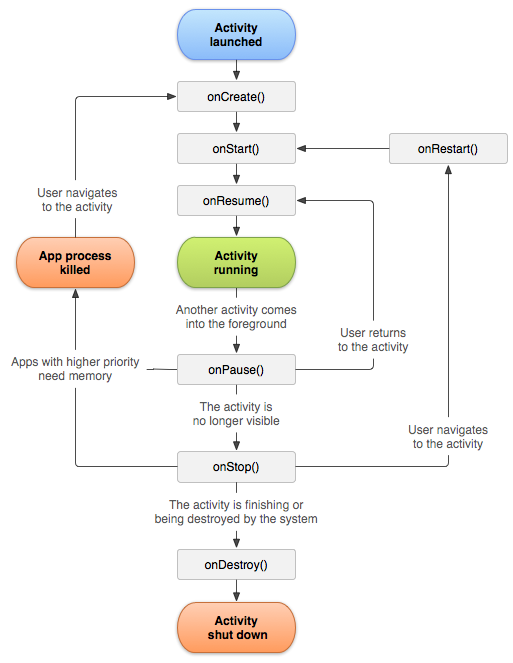
\includegraphics[scale=0.4]{04-framework/activity_lifecycle.png} 
   \caption{Ciclo de vida de una Activity}
   \label{fig:umlFrameworkCore}
\end{figure}


\section{Fragments}
Un Fragment representa una sección modular y reusable de la IU de una Activity, el cual se puede agregar o quitar mientras la Activity se esté ejecutando (algo así como una "sub-Activity"). Se pueden combinar varios Fragments en una sola Activity para crear una IU multipanel y volver a usar un Fragment en diferentes Activities.


Un Fragment define y administra su propio diseño, su propio ciclo de vida, y recibe sus propios eventos de entrada. Un Fragment no es un componente de app, por lo que no es un punto de entrada a la app como lo es una Activity. Un Fragment no puede "vivir" por si mismo, debe ser hospedado por una Activity, y el ciclo de vida del Fragment se ve afectado directamente por el ciclo de vida de la Activity anfitriona. Por ejemplo, cuando la Activity está pausada, también lo están todos sus Fragments, y cuando la Activity se destruye, lo mismo ocurre con todos los Fragments. Sin embargo, mientras una Activity se está ejecutando (está en el estado 'running' del ciclo de vida), se puede manipular cada Fragment de forma independiente, por ejemplo, para agregarlo o quitarlo. Cuando se realiza una transacción de Fragments como esta, también se pueden agregar a una pila administrada por la Activity; cada entrada de la pila de la Activity es un registro de la transacción de Fragments realizada. La pila le permite al usuario invertir una transacción de Fragments (navegar hacia atrás) al presionar el botón Atrás del dispositivo móvil.

El siguiente diagrama muestra los estados mas importantes por los que pasa un Fragment. Los rectángulos representan métodos de respuesta a llamada que se pueden implementar para realizar operaciones cuando el Fragment se mueve entre un estado y otro. Los óvalos representan los estados más importantes por los que pasa un Fragment.


\begin{figure}[H]
  \centering
    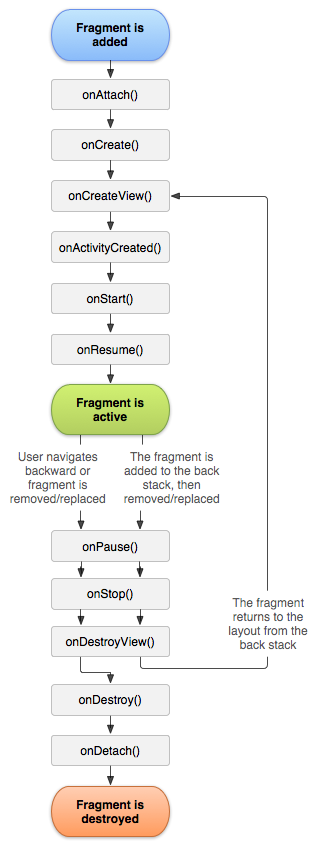
\includegraphics[scale=0.4]{04-framework/fragment_lifecycle.png} 
   \caption{Ciclo de vida de un Fragment}
   \label{fig:umlFrameworkCore}
\end{figure}


Los Fragments introducen modularidad y reusabilidad en la IU de una Activity, permitiendo dividir la IU en módulos más discretos. Se pueden usar múltiples instancias de un mismo Fragment en la misma Activity, en varias Avtivities, o incluso dentro de otro Fragment. Por esta razón se deben diseñar los Fragments solamente con la lógica necesaria para manejar su propia IU, de forma que sean independientes, evitando la dependencia con otros Fragments.
Con esto en mente, las Activities son el lugar ideal para poner los elementos globales de la IU, como por ejemplo una barra de navegación. Por el contrario, los Fragments son mejor lugar para definir y manejar la IU de una sola pantalla, o una sección de la misma.

Por ejemplo, en una app que responde a varios tamaños de pantalla, la app debería mostrar en pantallas pequeñas una barra de navegación con íconos y una lista lineal con el contenido. En cambio, en pantallas más grandes, debería mostrar un área de navegación más detallada y el contenido en forma de grilla para aprovechar mejor el espacio.
Administrar todas estas variaciones en la Activity puede resultar engorroso. Separar los elementos de navegación del contenido hace este proceso más manejable. La Activity es responsable de mostrar la IU de navegación correcta mientras que el Fragment muestra el contenido con la disposición adecuada.

\begin{figure}[H]
  \centering
    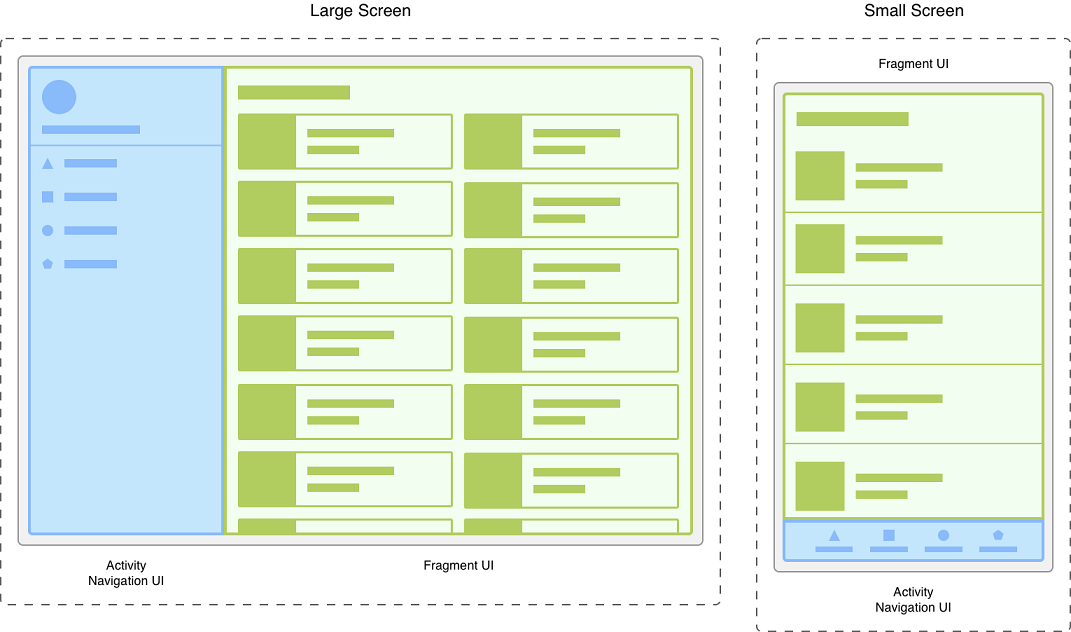
\includegraphics[scale=0.4]{04-framework/fragment-screen-sizes.png} 
   \caption{Dos versiones de la misma pantalla en diferentes tamaños de pantalla}
   \label{fig:umlFrameworkCore}
\end{figure}


Para crear un Fragment, se debe crear una subclase Fragment (o una subclase existente de ella). La clase Fragment tiene un código que se asemeja bastante a una Activity. Contiene métodos de devolución de llamada similares a los de una actividad, como onCreate(), onStart(), onPause() y onStop(), aunque agrega otros para controlar cuando se crea y destruye su IU, o cuando se adjunta el Fragment a la Activity anfitriona.
\cite{androidDocs}


\section{Services}
Un Service es un componente de app que puede realizar operaciones de larga ejecución en segundo plano y que no proporciona una interfaz de usuario. Una vez iniciado, un Service puede continuar ejecutándose en segundo plano aún cuando el usuario cambie a otra app. Además, un componente puede enlazarse con un Service para interactuar con él e incluso realizar una comunicación entre procesos (IPC por sus siglas en inglés). Por ejemplo, un Service puede manejar transacciones de red, reproducir música, realizar I/O de archivos o interactuar con un ContentProvider, todo en segundo plano.
Un Service se ejecuta en el subproceso principal del proceso que lo contiene; el Service no crea su propio subproceso ni se ejecuta en un proceso separado (a menos que se especifique lo contrario), por lo que parar realizar un trabajo que consume más CPU u operaciones de bloqueo (como reproducción MP3 o funciones de red), se debe crear un subproceso nuevo dentro del Service para completar ese trabajo.

Hay tres tipos de Service:

\begin{itemize}
	\item \textbf{Primer plano:} Un Service en primer plano realiza una operación que el usuario puede notar. Por ejemplo, una aplicación de audio usa un Service en primer plano para reproducir una pista de audio. Los Services en primer plano deben mostrar una notificación para que el usuario sea consciente de que el Service se está ejecutando. Estos Services continúan ejecutándose incluso si el usuario deja de interactuar con la aplicación.
	
	
	\item \textbf{Segundo plano:} Un Service en segundo plano realiza una operación que el usuario no nota directamente. Por ejemplo, si una aplicación usa un Service para comprimir su almacenamiento, suele tratarse de un Service en segundo plano.
	
	
	\item \textbf{Enlace:} Un Service es de enlace cuando un componente de app se vincula a él llamando a bindService(). Un Service de enlace ofrece una interfaz cliente-servidor que permite que los componentes interactúen con el Service, envíen solicitudes, reciban resultados e incluso lo hagan en distintos procesos con la comunicación entre procesos (IPC). Un Service de enlace se ejecuta solamente mientras otro componente de aplicación está enlazado a él. Se pueden enlazar varios componentes con el mismo Service a la vez, pero cuando todos ellos se desenlazan, el Service se destruye.
\cite{androidDocs}		
\end{itemize}




\section{BroadcastReceivers}
Las apps de Android pueden enviar o recibir mensajes de emisión desde el sistema de Android y otras apps para Android, de forma similar al patrón de diseño de publicación y suscripción. Estas emisiones se envían cuando ocurre un evento de interés. Por ejemplo, el sistema Android envía emisiones cuando ocurren diferentes eventos del sistema, como cuando este se inicia, cuando el dispositivo comienza a cargarse o cuando se conecta a una red de Internet. Las apps también pueden enviar emisiones personalizadas, por ejemplo, para notificar a otras apps sobre algo que podría interesarles (como cuando se descargaron algunos datos nuevos).
Las apps pueden registrarse para recibir emisiones específicas. Cuando se envía una emisión, el sistema redirige automáticamente las emisiones a las apps que se suscribieron para recibir ese tipo de emisión particular.
Un BroadcastReceiver es un componente de app que permite recibir esos mensajes de emisión, incluso si la app no se está ejecutando en ese momento, ya que estos mensajes se generan fuera del flujo de usuario habitual.
\cite{androidDocs}


\begin{comment}

\section{Permisos}
[aca falta describir como funcionan los permisos para acceder a las funciones sensibles del dispositivo móvil en Android...]

\end{comment}



\chapter{Samplers: Framework Android}

\section{Propuesta general}

\subsection{Descripción del problema}

Como se vio antes, se necesitaba de un entorno que permitiera a un científico poder crear una aplicación móvil con facilidad para poder incluir ciencia ciudadana en sus proyectos de ciencia ciudadana, mas precisamente, en proyectos de recolección.

La idea es que un científico pueda crear una aplicación móvil de ciencia ciudadana sin tener conocimientos de programación. Por ejemplo, desde una página web armar el protocolo de recolección de las muestras y con el mismo poder generar una aplicación móvil que sirva para tomar las muestras siguiendo dicho protocolo.

El protocolo de recolección estaría compuesto por los diferentes pasos necesarios para tomar la muestra con la aplicación. Estos pasos deben permitir:
\begin{itemize}
\item capturar una foto, un video o un audio.
\item tomar la posición del GPS o grabar un recorrido con el GPS.
\item contestar una pregunta con respecto a la muestra. Esta pregunta puede tener una o múltiples respuestas posibles.
\item introducir anotaciones (texto).
\item seleccionar una fecha o una hora.
\item mostrar información de orientación para la toma de la muestra.
\end{itemize}

Las muestras recolectadas con la aplicación deben ser enviadas por Internet a un servidor web previamente configurado para dicho propósito.

La aplicación generada debe ser una aplicación nativa, y no una solución web por ejemplo, para poder aprovechar mejor las características de los dispositivos móviles (cámara, GPS, etc.). Además se debe contemplar que al momento de tomar una muestra es posible que no se cuente con conexión a Internet, pero igualmente se debe permitir la toma de la muestra y se la debe almacenar en el dispositivo móvil hasta que haya conexión a Internet y pueda ser enviada al servidor web.

La aplicación generada servirá para tomar muestras siguiendo el protocolo de recolección especificado, almacenarlas y empaquetarlas en el dispositivo móvil hasta que puedan ser enviadas al servidor web.

Además se deberá contemplar algún mecanismo para poder mostrar ayuda para el usuario final de la aplicación (el científico ciudadano) que sirviera de orientación para tomar la muestra. 

También se debe contemplar algún mecanismo de identificación del usuario que toma las muestras, con usuario y contraseña, o con alguna red social (Facebook, Twitter, Instagram, Google, etc.) para así poder darle una devolución mostrándole información, o incentivarlo para que siga participando del proyecto a través de gamificación por ejemplo.



\subsection{Alcance de la solución propuesta}
En un principio, Samplers se pensó para que un científico pudiera crear su propia aplicación móvil de ciencia ciudadana sin tener conocimientos de programación. 
La idea inicial era que, mediante una aplicación web, el científico pudiera armar el protocolo de recolección de las muestras de manera visual e intuitiva, y se generara un archivo de configuración para Samplers. 
Con el archivo de configuración se pasaría a Samplers y se generaría la app para Android (el archivo APK para instalarla). 
Pero de esta forma el alcance de la tesis era muy grande, por lo que se decidió quitar la parte de la aplicación web y suponer que que el archivo de configuración ya viene armado.

Como se mencionó antes se requerían aplicaciones nativas, pero abarcar los 3 sistemas operativos móviles más usados en ese momento (Android, iOS y Windows Phone) era mucho para el alcance de esta tesis, por lo que se decidió optar por Android, que era el sistema operativo móvil más usado en ese momento. Según una estadística de Gartner sobre las ventas de smartphones a nivel mundial en el último trimestre de 2016\cite{gartner}, mas del 80\% de las mismas fueron de celulares con Android, y ese porcentaje fue creciendo hasta obtener una cuota del mercado del 88\% a nivel mundial a mediados de 2018. En la actualidad, en Argentina esa cuota de mercado es mas grande, llegando al 93\% según datos publicados por Carrier y Asociados en su reporte Mercado Celular Argentino 2019\cite{carrier}.

Para desarrollar aplicaciones móviles para la plataforma Android, el entorno de desarrollo integrado (IDE por sus siglas en inglés) oficial es Android Studio\cite{androidStudio}, por lo que Samplers se apoya sobre el mismo. Android Studio ha sido publicado de forma gratuita bajo Licencia Apache 2.0 y está disponible para las plataformas Microsoft Windows, MacOS y GNU/Linux.

\subsection{Descripción de la solución propuesta: Samplers}
Samplers es un framework que permite construir, de manera sencilla, aplicaciones Android (apps) para recolectar muestras en proyectos de Ciencia Ciudadana. Brinda una solución simple al problema de la recolección de la muestra aprovechando las funcionalidades de los dispositivos móviles.

Configurando el Workflow (que representa el protocolo de recolección en Samplers) y unos parámetros más, con Samplers se puede generar una app lista para ejecutarse en un dispositivo móvil Android. Esta app generada sirve para tomar muestras siguiendo el Workflow especificado, y las almacena en el dispositivo móvil hasta que puedan ser enviadas a un servidor web previamente configurado.

La app generada contiene, entre otras cosas, una Activity principal que muestra un texto de bienvenida (configurable) y un botón para tomar una muestra. Al presionar dicho botón se llama a la Activity encargada de tomar las muestras siguiendo el Workflow configurado. Esta Activity va mostrando en pantalla un Fragment por cada «paso» dentro del Workflow (Steps en Samplers). Cada uno de estos Fragments va interactuando con el usuario final de la app, el científico ciudadano\footnote{Se diferencia al usuario de Samplers, que es el que desea generar una app para recolectar muestras en un proyecto de ciencia ciudadana, del usuario final de la app, que es quien va a usar la app generada, que sería el científico ciudadano.}, para completar cada uno de los Steps del Workflow y así tomar la muestra (Sample en Samplers).

Para configurar el Workflow y los demás parámetros que necesita Samplers para generar la app, se debe completar un archivo de configuración llamado SamplersConfig.json.

Por ejemplo, si se desea crear una aplicación para hacer un relevamiento de las zonas con presencia del mosquito transmisor del Dengue (Aedes Aegypti), solicitando a los científicos ciudadanos que tomen fotos de los mosquitos que encuentren con las características del mosquito Aedes Aegypti, junto con la posición del GPS del dispositivo móvil. De esta manera se podría identificar al mosquito con la foto, y con la posición GPS armar un mapa de los avistajes. Para recolectar estas muestras se podría definir el protocolo de recolección de la siguiente manera:

\begin{enumerate}

\item Mostrar al científico ciudadano las características del mosquito Aedes Aegypti para que las pueda comparar con el mosquito encontrado (para evitar el envío de fotos innecesarias).

\item Pedir al científico ciudadano que tome una foto desde arriba del mosquito.

\item Pedir al científico ciudadano que tome una foto del costado del mosquito.

\item Pedir al científico ciudadano que tome la posición del GPS

\end{enumerate}

Para representar este protocolo de recolección se debería configurar el Workflow en el archivo de configuración para Samplers de la siguiente manera: 

\begin{figure}[H]
  \centering
    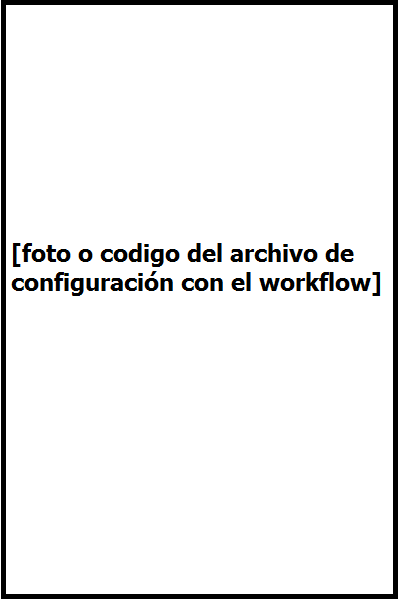
\includegraphics[scale=0.8]{05-implementacion/archivo_config_ejemplo.png} 
   \caption{Archivo de configuración para Samplers de la app ejemplo}
\end{figure}


Con este archivo de configuración, Samplers generará el código necesario para la app, que al compilarla y ejecutarla en un dispositivo móvil Android se verá como muestra la siguiente imagen:


\begin{figure}[H]
  \centering
    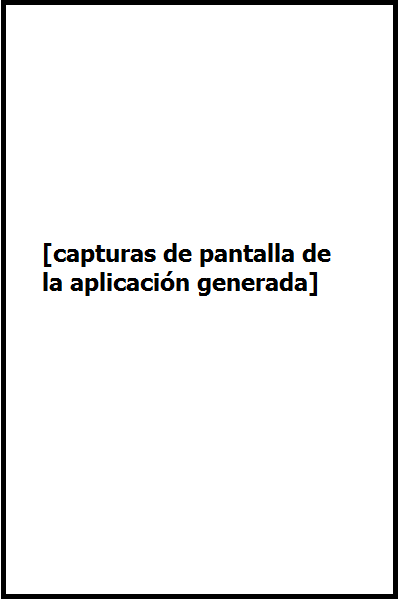
\includegraphics[scale=0.8]{05-implementacion/app_generada_ejemplo.png} 
   \caption{Capturas de pantalla de la app de ejemplo generada por Samplers}
\end{figure}


Las opciones disponibles y cómo se configura el archivo de configuración de Samplers se explican en la sección \ref{sec:archivo_configuracion}.

De esta manera un científico que desee generar una app para su proyecto de ciencia ciudadana, solo tiene que completar el archivo de configuración, ejecutar Samplers y luego compilar en Android Studio y ejecutar la app en un dispositivo móvil o en los dispositivos virtuales que provee Android Studio para debugging.

Como Samplers genera el código fuente de la app, esto permite que un usuario con conocimientos de programación pueda modificarlo y personalizar la app a su gusto, así como también agregarle otras funcionalidades a la app generada. También permite que pueda ser usado en una app ya desarrollada o en desarrollo, como si fuera una librería que se incluye al proyecto y permite usar sus clases (esto se explica con más detalle en la sección \ref{sec:usando_las_clases}).

Como Samplers se pensó como un proyecto dentro de Cientópolis\cite{cientopolis} el mismo es open source y se usó un repositorio público en GitHub\cite{github} para dejar el código fuente disponible para todo el mundo.


\begin{comment}
También provee un mecanismo de identificación del usuario final de la aplicación (el científico ciudadano) usando su cuenta de Google, ya que en los dispositivos móviles con sistema operativo Android se requiere de una cuenta de Google para acceder a muchas de las funcionalidades, como por ejemplo la Play Store (la tienda de Android para descargar aplicaciones).  Ademas esta preparado para que el usuario del framework pueda incluir su propio sistema de inicio de sesión (por ejemplo con usuario y contraseña) o con una API de alguna red social, como Facebook, Twitter, Instagram, etc.


Samplers también provee un mecanismo para mostrar ayuda asociada a un paso (Step) en particular y una ayuda general en la pantalla principal, usando archivos HTML. Se optó por los mismos por la variedad de opciones y posibilidades que conllevan, y por su simpleza para mostrarlos.
\end{comment}

\subsection{Archivo de configuración}\label{sec:archivo_configuracion}

\begin{comment}

En el objeto project, se encuentran las configuraciones del proyecto de Android Studio en el cual se creará la app, y son las siguientes:
\begin{itemize}

\item app\_path: la ruta relativa a los archivos fuente de la app. Es donde se crearán los archivos de las Activities por ejemplo.

\item package\_name: el nombre del package que se usará para las Activities de la app (generalmente ``com.example.myApplication"). 

\end{itemize}

En el objeto application, se encuentran los parámetros para configurar la app, como por ejemplo el mensaje de bienvenida o el servidor web al que se deben enviar las muestras recolectadas. Los parámetros son los siguientes:
\begin{itemize}

\item title: el título de la app.

\item welcomeMessage: el mensaje de bienvenida que se muestra en la Activity principal.  

\item networkConfiguration: la configuración del servidor al que se enviarán las muestras tomadas con la app

\begin{itemize}
\item url: la url del servidor a la cual se enviarán las muestras mediante un mensaje HTTP POST.

\item paramName: el nombre del parámetro dentro del mensaje HTTP POST que se usará para enviar la muestra.

\item paramNameUserId: [Opcional] el nombre del parámetro dentro del mensaje HTTP POST que se usará para enviar el id del usuario que tomó la muestra (si los métodos de identificación estan habilitados).

\item paramNameAuthenticationType: [Opcional] el nombre del parámetro dentro del mensaje HTTP POST que se usará para enviar el tipo de identificación que se usó (si los métodos de identificación estan habilitados).

\end{itemize}

\item googleMaps\_API\_KEY:

\item mainHelpFileName: [Opcional] se puede espe 
el nombre del archivo HTML que se usará.
The file name of the HTML file containing the main application help

\item authenticationEnabled: [Opcional] habilita los métodos de identificación del usuario que toma las muestras.

\item authenticationOptional: [Opcional] indica si la identificación (en caso de estar habilitada) será opcional u obligatoria.


\end{itemize}

\end{comment}

El archivo de configuración es un archivo en formato JSON que se debe completar con los parámetros necesarios para crear la app con Samplers. Se eligió el formato JSON porque nos pareció más sencillo de manipularlo por una persona (que XML por ejemplo, que también fue evaluado), suponiendo que el científico tuviese que editarlo manualmente.

El archivo está compuesto por tres objetos: project, application y workflow.

En el objeto project, se encuentran las configuraciones del proyecto de Android Studio en el cual se creará la app, como por ejemplo la ruta en donde se crearán los archivos de las Activities y el nombre del package que se usará para las mismas. 

En el objeto application, se encuentran los parámetros para configurar la app, como por ejemplo el título de la app, el mensaje de bienvenida o el servidor web al que se deben enviar las muestras recolectadas. 

El objeto workflow se usa justamente para configurar el Workflow (el protocolo de recolección) que usará la app para tomar las muestras. En el mismo se deben especificar los Steps que se usarán con sus respectivos parámetros cada uno. Por defecto Samplers provee los siguientes Steps:

\begin{itemize}

\item Information: Muestra un texto al científico ciudadano.

\item Photo: Solicita tomar una foto.

\item Sound: Solicita grabar sonido.

\item Location: Solicita tomar la posición del GPS del dispositivo móvil.

\item Route: Solicita grabar con el GPS del dispositivo móvil un recorrido (un conjunto de posiciones GPS).

\item SelectOne: Solicita seleccionar una única respuesta a una pregunta.

\item MultipleSelect: Solicita seleccionar una o varias respuestas a una pregunta.

\item InsertText: Solicita ingresar texto.

\item InsertDate: Solicita seleccionar una fecha.

\item InsertTime: Solicita seleccionar una hora.

\end{itemize}

En la siguiente imagen se muestra un ejemplo del archivo de configuración para Samplers.
\begin{figure}[H]
  \centering
    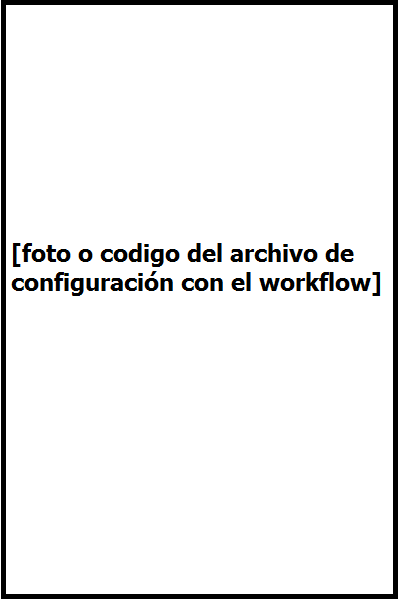
\includegraphics[scale=0.8]{05-implementacion/archivo_config_ejemplo.png} 
   \caption{Ejemplo de un archivo de configuración para Samplers}
\end{figure}

Una vez configurado el archivo, Samplers generará una Activity principal para la app que tendrá todas las configuraciones del objeto application y que usará el Workflow configurado para llamar a la Activity encargada de tomar las muestras (TakeSampleActivity) cuando el científico ciudadano presione el botón para tomar una muestra.

El detalle de todos los parámetros, como configurar el archivo de configuración y los diferentes Steps disponibles para armar el Workflow se explican en la sección \ref{sec:archivo_config_detallado}


\subsection{Usando las clases} \label{sec:usando_las_clases}

[Aca explicaremos cómo sería usando las clases (para una app existente por ejemplo), pero sencillo y por arriba porque todavia no se explicaron las clases en detalle que viene en la siguiente sección].

\section{Estructura del Framework}

************************************


Samplers está compuesto por dos elementos: una librería con las clases y [demases (activities, fragments, recursos)] necesarias para crear la app y un script en Gradle para procesar el archivo de configuración.

La libreria es un archivo .aar, que es similar a un archivo .jar de Java, pero especifico para Android. En el mismo están todas las clases y los archivos de recursos del framework.

************************************


A continuación se explican las clases que permiten que se cree una aplicación móvil con Samplers y su funcionamiento.

\subsection{Workflow, Step, StepFragment, StepResult, Sample}
Estas clases conforman el corazón del framework, y son las necesarias para poder definir el protocolo de recolección de las muestras.

A continuación se muestra el diagrama de clases (Figura \ref{fig:umlFrameworkCore}).

\begin{figure}[H]
  \centering
    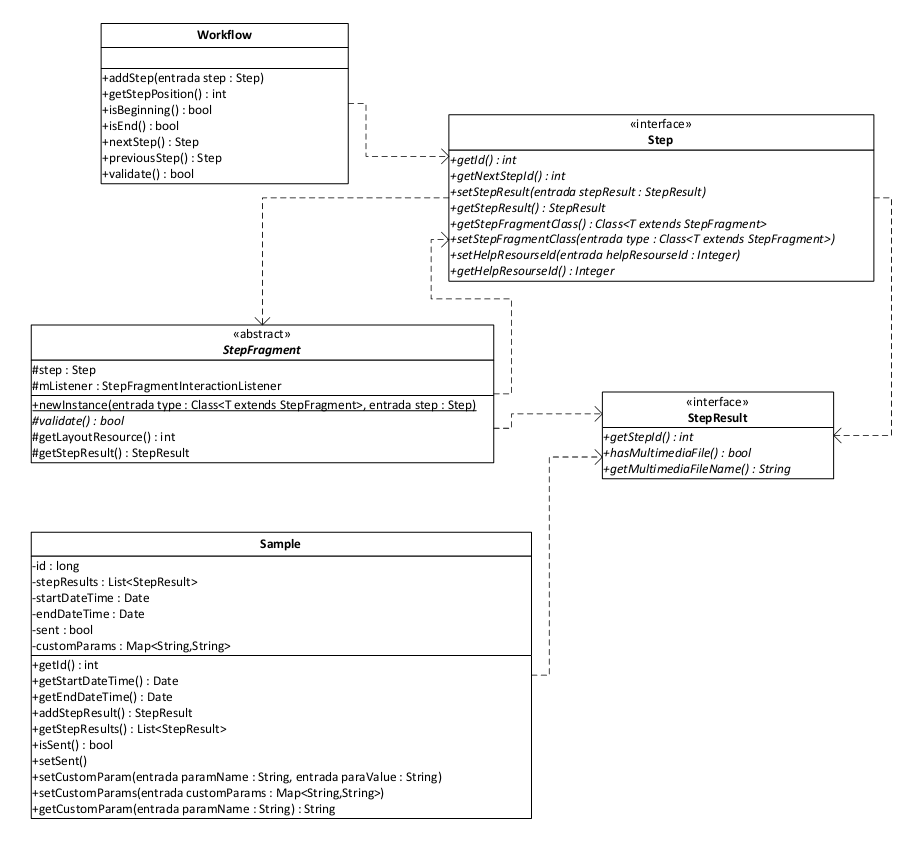
\includegraphics[scale=0.4]{05-implementacion/FrameworkCore.png} 
   \caption{Diagrama de clases del core del framework}
   \label{fig:umlFrameworkCore}
\end{figure}


TakeSampleActivity es una Activity y es la encargada de tomar la muestra.
Recibe como parámetro un Workflow, que representa el protocolo de recolección de la muestra.
El Workflow esta formado por varias instancias de Step, que representan cada una un paso a seguir dentro del protocolo de recolección para obtener la muestra.

TakeSampleActivity ejecuta el Workflow y por cada Step obtiene y muestra en pantalla el StepFragment asociado, que es el Fragment encargado de mostrar la interfaz de usuario para ejecutar ese Step. 
El StepFragment a través de la interacción con el usuario final (el científico ciudadano) genera un StepResult, que es el resultado de la ejecución del Step asociado. Por cada tipo de Step, debe haber una clase StepFragment que sepa ejecutar ese Step y generar el StepResult asociado.

El conjunto de todos los StepResults obtenidos después de ejecutar todos los Steps del Workflow forman la muestra, que esta representada por la clase Sample.


\subsubsection{Workflow: el protocolo de recolección de las muestras}
La clase Workflow representa el protocolo de recolección de las muestras. Está formado por una colección de Steps, que representan los pasos a seguir para completar dicho protocolo, y un Step inicial que indica el inicio del mismo (el primer Step a ejecutar).

El Workflow es el encargado de llevar el estado del paso en el que se encuentra, y posee métodos para obtener el siguiente Step (\textit{nextStep()}  que depende del Step actual) y el Step anterior (\textit{previuosStep()}  para lo que maneja una lista a modo de pila\footnote{Stack en inglés, una lista ordenada con acceso a sus elementos de tipo «último en entrar, primero en salir»}).

El Workflow se comporta de manera secuencial, puede ir hacia adelante o volver hacia atrás, pero esto no impide que pueda tener bifurcaciones, y así formar diferentes caminos para tomar la muestra. Por ejemplo, se le podría preguntar al científico ciudadano si observa una característica particular al momento de tomar la muestra, y si la observa solicitarle que tome una foto de la misma, pero en caso contrario se puede omitir el paso de la foto.

\subsubsection{Step: el paso}
Un Step representa un paso dentro del Workflow. Tiene asociado un StepFragment que es el encargado de ejecutar el Step para generar un StepResult (el resultado). El Step básicamente tiene los parámetros o información para que pueda ser ejecutado por el StepFragment.
Por ejemplo, para el caso en que el paso sea contestar una pregunta, el Step tendrá la pregunta en sí (un String) y una colección con las posibles respuestas (id y descripción).

El Step conoce cuál es el siguiente Step a ejecutar aunque a veces éste depende del StepResult generado, como es el caso de SelectOneStep en el que el siguiente paso depende de la opción seleccionada, y con esto se pueden crear bifurcaciones en el Workflow.

Samplers provee los siguientes Steps:
\begin{itemize}
	\item InformationStep: Muestra una información (texto) al usuario.
	\item PhotoStep: Permite tomar una foto con la cámara del dispositivo móvil.
	\item SoundRecordStep: Permite grabar un sonido con el micrófono del dispositivo móvil.
	\item SelectOneStep: Muestra una pregunta con varias opciones como respuesta, de las cuales solo se puede seleccionar una sola.
	\item MultipleSelectStep: Muestra una pregunta con varias opciones como respuesta, de las cuales solo se pueden seleccionar varias opciones.
	\item LocationStep: Permite tomar la geo posición del dispositivo móvil.
	\item RouteStep: Permite grabar un recorrido usando el GPS del dispositivo móvil.
	\item InsertTextStep: Permite ingresar un texto.
	\item InsertDateStep: Permite seleccionar una fecha.
	\item InsertTimeStep: Permite seleccionar una hora.
\end{itemize}

El detalle de estos Steps y su funcionamiento se explican en la sección \ref{sec:steps_detallados}.

Si bien estos son los Steps que provee Samplers de manera predeterminada, un usuario programador puede definir y agregar sus propios Steps, junto con sus StepFragments y StepResults como se explica en la sección \ref{sec:definir_steps}.

\subsubsection{StepFragment: la vista y controlador del Step}
El StepFragment es el encargado de ejecutar un Step y generar un StepResult con la interacción del usuario final (el científico ciudadano). Un StepFragment recibe un Step, que generalmente contiene los parámetros necesarios para ejecutarlo, y en base a eso muestra un Fragment para que, interactuando con el científico ciudadano, poder obtener un resultado (StepResult) para la muestra (Sample). 

Por ejemplo, para el caso en que el paso sea contestar una pregunta, se mostrará la pregunta y se listarán las posibles respuestas en forma de radio-buttons, si solo se admite seleccionar una única respuesta, o en forma de check-buttons, si se permite seleccionar más de una.

Por cada tipo de Step, debe haber una clase StepFragment que sepa ejecutar ese Step y generar el StepResult asociado.

Es una clase abstracta, ya que su comportamiento depende de la implementación de cada tipo de StepFragment que se defina. Se definió así y no como una interfaz por la necesidad de que heredara de Fragment porque así lo necesita la Activity TakeSampleActivity, que es la encargada de ejecutar el Workflow para tomar la muestra.

Por cada Step que provee Samplers de manera predeterminada, también se provee un StepFragment que ejecuta cada Step. Asimismo, un usuario programador también puede desarrollar un StepFragment propio para alguno de los Steps provistos por Samplers, como se explica en la sección \ref{sec:definir_steps}



\subsubsection{StepResult: el resultado de la ejecución de un Step}
El StepResult representa el resultado que se obtiene de ejecutar un Step. Contiene los datos obtenidos de ejecutar el Step asociado. Cada ejecución de un mismo Step, puede generar un StepResult diferente.

Por ejemplo, para el caso en que el Step sea contestar una pregunta, el StepResult contendrá la respuesta seleccionada, si solo se admite seleccionar una única respuesta, o una colección de respuestas, si se permite seleccionar más de una.

Se definió como una interfaz, ya que su comportamiento depende de la implementación de cada tipo de Step que se defina.

Un StepResult tiene asociado el Step en base al cual se generó. También puede tener asociado un archivo multimedia, como por ejemplo en los casos de PhotoStep y SoundRecordStep que guardan una foto y un archivo de sonido respectivamente.


\subsubsection{Sample: la Muestra}
La clase Sample representa una muestra tomada a partir de seguir los pasos (Steps) del protocolo del recolección (Workflow). Contiene los resultados (StepResult) de la ejecución de cada paso. Cada ejecución del Workflow puede generar una colección de StepResults diferente.

También guarda fecha y hora de inicio y finalización. Esto es útil para sacar una estadística de cuanto tarda un científico ciudadano en recolectar una muestra y así poder analizar optimizaciones para la aplicación final.

Una vez recolectadas, las muestras se guardan en el dispositivo móvil y son enviadas a través de Internet a un servidor web previamente configurado.

\subsection{TakeSampleActivity}
La clase TakeSampleActivity es la encargada de ejecutar el Worflow para tomar la muestra. Es una Activity que recibe un objeto Workflow como parámetro y va iterando sobre los Steps del mismo. A cada Step le pide su StepFragment y lo muestra en pantalla para que, interactuando con el científico ciudadano, se genere el StepResult para la muestra (Sample). Una vez finalizado el Workflow, guarda la muestra, controla si se puede enviar la misma y finaliza.



\subsection{Persistencia local}
Las muestras se guardan en el dispositivo móvil en un archivo JSON, junto con los archivos multimedia que pudiera tener, dentro de un directorio por cada muestra. Las mismas se guardan dentro del directorio samples en el almacenamiento interno del dispositivo.

Se eligió el almacenamiento interno para guardar las muestras porque no se necesitan permisos especiales para acceder al mismo y, de forma predeterminada, los archivos que se guardan en el mismo son privados para la aplicación y otras aplicaciones no pueden tener acceso a ellos (tampoco el usuario). Cuando el usuario desinstala la aplicación, estos archivos se quitan\cite{androidInternalStorage}.

Por ejemplo, una muestra con id 123456 y 2 fotos se guarda de la siguiente manera:
\begin{lstlisting}[language=Java, frame=tlb]
/samples/		// Directorio de muestras
  sample_123456/	// Directorio de la muestra con id:123456 
    sample_123456.json	// Objeto Sample en formato JSON
    1524437599776.jpg	// Archivo de foto 1
    1524441664170.jpg	// Archivo de foto 2
\end{lstlisting}

Para pasar la muestra a un archivo JSON se usó Gson\cite{gson}, una librería de Google distribuida bajo licencia Apache 2.0 que convierte objetos Java a JSON y viceversa de manera muy sencilla, con métodos \textit{toJson()} y \textit{fromJson()} para convertir hacia y desde JSON respectivamente.

\subsection{Envío de muestras a servidor web}

Una vez guardadas localmente, las muestras se envían al servidor web previamente configurado, mediante un mensaje HTTP POST. Para ello se usó la librería OkHttp\cite{okhttp}, distribuida por Square Inc. bajo licencia Apache 2.0, que resuelve de manera sencilla y eficiente el envío de mensajes HTTP en Android.

Por cada muestra se envía el objeto Sample en formato JSON junto con los archivos multimedia que pudiera tener, todo comprimido en un solo archivo ZIP. Para comprimir las mismas se usaron las librerías estándares de Java (java.util.zip) que proporciona clases para leer y escribir archivos ZIP y GZIP estándares.

Las muestras se envían automáticamente cuando se detecta conexión wifi o a petición del usuario usando cualquier red disponible.

Para el envío automático, se controla luego de guardar la muestra si hay conexión wifi y se intenta enviar la muestra; caso contrario queda pendiente de envío y se intenta enviar cuando se detecta conexión wifi. Para detectar la conexión a wifi se usa un BroadcastReceiver que atiende el evento de difusión que envía Android cuando el dispositivo móvil se conecta a wifi, aún cuando la app no se esté ejecutando, lo que permite el envío de la muestra con un Service en segundo plano.

Para el caso que es a petición del usuario, se listan las muestras tomadas en la Activity SamplesListActivity con un botón que permite el envío de las mismas usando cualquier tipo de conexión a Internet.

\subsection{Identificación}
Samplers provee un sistema de identificación (login), el cual se puede habilitar o no de acuerdo a las necesidades del proyecto. Si se habilita el mismo puede ser opcional, permitiendo al científico ciudadano tomar y enviar muestras habiéndose o no identificado, o puede ser obligatorio, requiriendo que el científico ciudadano se identifique para poder tomar y enviar las muestras.

De manera predeterminada Samplers incluye identificación con la API de Google, es decir que el científico ciudadano puede usar su cuenta de Google que tiene configurada en el dispositivo móvil Android para identificarse en la aplicación.

Además, un usuario programador del framework puede definir su propio método de identificación, ya sea con usuario y contraseña o usando alguna otra API de redes sociales por ejemplo, como son Facebook, Instagram, Twitter, etc. como se explica en la sección \ref{sec:usar_auth_propia}.

Cuando se envía la muestra también se incluyen dos parámetros que son el id del usuario identificado y el método usado para identificar (que puede ser google o uno personalizado). Se envían de esta forma porque al momento de tomar la muestra el científico ciudadano puede no estar identificado, e identificarse antes de enviarlas.

\subsection{Resto de la UI?? ANALIZAR}


\subsubsection{SamplersMainActivity}

\subsubsection{SamplesListActivity}


\subsubsection{HelpActivity}



\section{Instalación del framework}
En esta sección se describe como instalar el framework en Android Studio; se detallan los requisitos y los pasos a seguir para la instalación.

\subsection{Requerimientos mínimos:}

\begin{itemize}
\item Android Studio (Java): Si bien esta pensado para y probado en Android Studio, podria funcionar bien en otro entorno que use Java y deje importar archivos Android Archive (.aar).
\item Android SDK API17: Android 4.2 (Jelly Bean) o superior.
\end{itemize}

\subsection{Pasos para la Instalación:}

\begin{enumerate}
	\item Crear en Android Studio un nuevo proyecto vacío (sin ninguna Activity).
		\begin{itemize}
		\item Seleccionar API17 o superior como versión mínima de Android SDK
		\end{itemize}
	\item Importar la librería del framework en el proyecto creado
		\begin{itemize}
		\item Descargar la última versión de \textbf{samplersFramework.aar} desde https://github.com/cientopolis/samplers/releases/
		\item Importar la librería al proyecto: File -$>$ New -$>$ New Module -$>$ Import .JAR/.AAR Package
		\end{itemize}
	\item Agregar el repositorio de Google
		\begin{itemize}
			\item En el archivo build.gradle del proyecto agregar: 
			\begin{lstlisting}[language=XML, frame=single]
allprojects {
    repositories {
        jcenter()
        google()
    }
}
			\end{lstlisting}	
		\end{itemize}
	\item Agregar las dependencias necesarias:
		\begin{itemize}
			\item En el archivo build.gradle de la aplicación agregar: 
			\begin{lstlisting}[language=XML, frame=tlb]
dependencies {
  // acá estarían las dependencias predeterminadas creadas por Android Studio:
  // ...

  // si no son agregadas automáticamente, agregar las siguientes dependencias:
  // (se deberían agregar las de la ultima versión disponible)
  compile 'com.android.support:design:24.2.1' 
  compile 'com.android.support.constraint:constraint-layout:1.0.2'

  // para usar mapas y los servicios de geolocalización se deben agregar las 
  // siguientes dependencias (usar la ultima versión disponible)
  compile ('com.google.android.gms:play-services-location:12.0.1')
  compile ('com.google.android.gms:play-services-maps:12.0.1')
  
  // para usar autenticación con Google se deben agregar las 
  // siguientes dependencias (usar la ultima versión disponible)  
  compile ('com.google.android.gms:play-services-auth:12.0.1')

  // agregar la dependencia del framework Samplers
  compile project(":samplersFramework")
}
			\end{lstlisting}	
		\end{itemize}	

	\item Instanciar:
		\begin{itemize}
		\item La instanciación puede ser manual o usando el generador de clases en Gradle como se explica en la siguiente sección.
		\end{itemize}
\end{enumerate}	

\section{Instanciación y uso del framework}
En esta sección se explica como instanciar el framework para su uso, brindando algunos ejemplos concretos.

Una vez instalado el framework el siguiente paso es instanciarlo para usarlo. La instanciación puede ser manual o usando el generador de clases de Gradle.


\subsection{Instanciación manual}
Básicamente se tiene que crear un objeto Workflow, agregarle los objetos Steps, y llamar a la activity TakeSampleActivity pasándole el workflow como parámetro.
También es necesario establecer la configuración general en el método onCreate de la activity principal (main activity).
Se puede usar una activity principal propia o se puede heredar de SamplersMainActivity. En ambos casos se debe hacer lo siguiente:
\begin{itemize}
	\item Establecer la configuración general en el método onCreate de la activity principal:
		\begin{lstlisting}[language=Java, frame=tlb]
NetworkConfiguration.setURL("http://192.168.1.10/samplers/upload.php");
NetworkConfiguration.setPARAM_NAME_SAMPLE("sample");

// Opcional, si se desea usar autenticación (*)
NetworkConfiguration.setPARAM_NAME_USER_ID("user_id");
NetworkConfiguration.setPARAM_NAME_AUTHENTICATION_TYPE("authentication_type");

AuthenticationManager.setAuthenticationEnabled(true);
AuthenticationManager.setAuthenticationOptional(true);
		\end{lstlisting}
(*) Ver la sección \ref{sec:usando_autenticacion} para más detalles sobre como usar Autenticación.


	\item Crear un Workflow. Si se está heredando de SamplersMainActivity se debe hacer sobreescribiendo el método getWorkflow.
		\begin{lstlisting}[language=Java, frame=tlb]
@Override
protected Workflow getWorkflow() {
  Workflow workflow = new Workflow();
    	
  Step step = new InformationStep(2,"Por favor tome una foto de su gato", null);
  workflow.add(step);
    	
  step = new PhotoStep(1,"Bienvenido a la app de prueba", 2);
  workflow.add(step);
    	
  return workflow;
}		
		\end{lstlisting}
Nota: en el ejemplo anterior se muestra un Workflow que tiene dos Steps. El primero muestra un mensaje de bienvenida y el segundo pide para tomar una foto. Para ver los distintos Steps que se pueden usar vea la sección \ref{sec:steps_detallados}.

	\item Iniciar la activity TakeSampleActivity. Si se está heredando de SamplersMainActivity esto se hace automáticamente en el método onClick del botón "tomar muestra". De lo contrario, deberá iniciarla de la siguiente forma, en el método onClick de un botón por ejemplo:
		\begin{lstlisting}[language=Java, frame=tlb]
@Override
public void takeSampleClick(View view) {
  Workflow workflow = getWorkflow();

  Intent intent = new Intent(this, TakeSampleActivity.class);        
  intent.putExtra(TakeSampleActivity.EXTRA_WORKFLOW, workflow);
  startActivity(intent);
}		
		\end{lstlisting}

\end{itemize}


\subsection{Instanciación usando el  generador de clases de Gradle}

Básicamente, el generador de clases de Gradle se encarga de hacer una instanciación manual a partir de un archivo de configuración (JSON). Está pensado para desarrolladores que no tienen muchos conocimientos en Android, o para servir de interfaz entre una aplicación que genere apps a través de Samplers (***esto hay que escribirlo mejor***).

Los pasos para usar el generador de clases de Gradle son:
\begin{enumerate}
	\item Crear un archivo JSON con el nombre SamplersConfig.json
		\begin{itemize}
			\item El formato y las opciones están explicadas sección \ref{sec:archivo_config_detallado}.
			\item Para validar sintaxis se puede usar por ejemplo el validador online https://jsonformatter.curiousconcept.com que es gratuito.
			\item Al final de esta sección se provee un archivo de ejemplo.
		\end{itemize}
		
	\item Copiar el archivo creado en el item anterior al directorio raíz del proyecto Android creado.
	
	\item Descargar la última versión de los archivos \textbf{samplers.gradle} y \textbf{samplersclassgenerator.jar} del repositorio de Samplers (https://github.com/cientopolis/samplers/releases/) y copiarlos también al directorio raíz del proyecto Android.
	
	\item Enlazar el archivo samplers.gradle en el archivo \textbf{build.gradle} de la aplicación:
		\begin{itemize}
			\item Android Studio crea por defecto dos archivos build.gradle, uno a nivel de aplicación y otro a nivel de proyecto. Debe usarse el de aplicación.
			\item Al final del archivo build.gradle de aplicación agregar:
\begin{lstlisting}[language=XML, frame=tlb]
apply from: '../samplers.gradle'
\end{lstlisting}
			\item Al guardar los cambios, Android Studio sugerirá hacer una sincronización del proyecto, hacerla. Esto generará en la aplicación una activity llamada MyMainSamplersActivity en base a las opciones configuradas en el archivo SamplersConfig.json.
			\item Si se necesita volver a generar esta activity (si se quieren modificar algunas opciones por ejemplo ) se puede eliminar la misma, hacer las modificaciones en el archivo SamplersConfig.json y volver a generar el proyecto (en el menu Build -$>$ Make Project)
		\end{itemize}
		
	\item Eliminar o personalizar el archivo \textbf{style.xml} que está en \textbf{res/values} en la aplicación
	
	\item Ejecutar la aplicación y listo.

\end{enumerate}


\subsection{Secciones del Archivo} \label{sec:archivo_config_detallado}

El archivo SamplersConfig.json es un archivo JSON con 3 objetos:
\begin{itemize}
	\item El objeto \textbf{project}
		
	El objeto project tiene dos campos
	\begin{itemize}
		\item \textbf{app\_path}: Un String con la ubicación del directorio de los fuentes de la aplicación, relativo al directorio del proyecto. Es donde están los archivos -java de la aplicación y donde se creará el archivo MyMainSamplersActivity.java
		\item \textbf{package\_name}: Un String con el nombre del package usado para las activities de la aplicación. Es el package donde la activity MyMainSamplersActivity será agregada.
	\end{itemize}
	
Ejemplo:
\begin{lstlisting}[language=XML, frame=tlb]	
{
  "project" : {
    "app_path" = "app/src/main/java/com/example/myApplication/"
    "package_name" : "com.example.myApplication"
  }
}
\end{lstlisting}	
	
	\item El objeto \textbf{application}
	El objeto application tiene 7 campos, de los cuales 3 son requeridos y los otros 4 opcionales (para habilitar características especiales)
	\begin{itemize}
		\item \textbf{title}: Un String con el nombre de la aplicación.
		
		 \item \textbf{welcomeMessage}: Un String con el mensaje de bienvenida que se mostrará en la activity principal (MyMainSamplersActivity)
		 
		 \item \textbf{networkConfiguration}: Un objeto con la configuración de red que se usará para enviar las muestras al servidor web. Ver mas abajo la configuración de este objeto.
		 
		 \item \textbf{googleMaps\_API\_KEY}: [Opcional] Un String con la API Key de Google. Este campo es necesario si se van a usar los servicios de ubicación y mapas (Location Step y Route Step). La API Key de google se puede obtener desde la página de google developers (https://developers.google.com/maps/documentation/android-api/signup)
		 
		 \item \textbf{mainHelpFileName}: [Opcional] Un String con el nombre del archivo HTML que contiene la ayuda principal de la aplicación. Este archivo debe estar junto con el archivo SamplersConfig.json. Ver la sección Mostrando Ayuda para mas detalles.
		 
		 \item \textbf{authenticationEnabled}: [Opcional] Un boolean que indica si se usará autenticación (true) o no (false). Si se omite este campo se asume false. Ver la sección Usando Autenticación para mas detalles.
		 
		 \item \textbf{authenticationOptional}: [Opcional] Un boolean que indica si la autenticación será opcional (true) o requerida (false). Si se omite este campo se asume true (autenticación opcional). Este campo solo tiene sentido si se usa autenticación. Ver la sección Usando Autenticación para mas detalles.
		 
	\end{itemize}
	
	
	El objeto \textbf{networkConfiguration}:
	El objeto networkConfiguration contiene la configuración de red que se usará para enviar las muestras al servidor web. Tiene 4 campos, de los cuales 2 son requeridos y los otros 2 opcionales.
	
	\begin{itemize}
	
		\item \textbf{url}: Un String con la URL del servidor web al cual se le enviaran las muestra con un mensaje HTTP POST.
		
		\item \textbf{paramName}: Un String con el nombre del parámetro dentro del mensaje HTTP POST en el que se enviará la muestra.
	
		\item \textbf{paramNameUserId}: (Opcional) Un String con el nombre del parámetro dentro del mensaje HTTP POST en el que se enviará el id del usuario que envía la muestra. Este campo solo es necesario si se usa autenticación. Ver la sección Usando Autenticación para mas detalles.
		
		\item \textbf{paramNameAuthenticationType}: (Opcional) Un String con el nombre del parámetro dentro del mensaje HTTP POST en el que se enviará el tipo de autenticación que usó el usuario que envía la muestra. Este campo solo es necesario si se usa autenticación. Ver la sección Usando Autenticación para mas detalles.
	
	\end{itemize}
	
	
Ejemplo:
\begin{lstlisting}[language=XML, frame=tlb]
{
  "application": {
    "title" : "Samplers Hello World App",
    "welcomeMessage" : "Welcome to your first Samplers App!",
    "networkConfiguration" : {
      "url" : "http://192.168.1.10/samplers/upload.php",
      "paramName" : "sample",
      "paramNameUserId" : "user_id",
      "paramNameAuthenticationType" : "authentication_type"
    },
    "authenticationEnabled" : true,
    "authenticationOptional" : true,
    "googleMaps_API_KEY" : "your_google_maps_API_KEY",
    "mainHelpFileName" : "mainhelp.html"
  } 
}
\end{lstlisting}	
	
	
	\item El objeto \textbf{workflow}
	El objeto workflow representa el protocolo para la toma de la muestra. Son los pasos que se ejecutarán para tomar la misma.
	El objeto cuenta con dos campos:
		
	\begin{itemize}
	
		\item \textbf{actionLabel}: Un String con el título que se usará para el botón que inicia la activity TakeSampleActivity, que es la encargada de tomar la muestra.
		
		\item \textbf{steps}: Un Array de Objetos Step los cuales forman el workflow. El primer objeto del array se considera como el inicio del mismo. Ver la sección Steps para mas detalles.
	
	
	\end{itemize}	
	
	
Ejemplo:
\begin{lstlisting}[language=XML, frame=tlb]	
{
  "workflow": {
    "actionLabel" : "Tomar muestra",
    "steps": [
      {
        "id" : 1,
        "type" : "Information",
        "text" : "Por favor, siga las instrucciones",
        "nextStepId" : 2
      },
      {
        "id" : 2,
        "type" : "Location",
        "text" : "Por favor posicione la muestra en el mapa",
        "nextStepId" : 3,
        "helpFileName" : "locationhelp.html"
      },
      {
        "id" : 3,
        "type": "MultipleSelect",
        "title" : "Seleecione las cosas que ve",
        "helpFileName" : "selecthelp.html",
        "options" : [
          {
            "id":1,
            "text":"Arboles"
          },
          {
            "id":2,
            "text":"Basura"
          },
          {
            "id":3,
            "text":"Agua"
          }
        ]
      }
    ]
  }
}

\end{lstlisting}	
	
\end{itemize}

**FALTA DESARROLLAR**

Aca podriamos poner un ejemplo completo de un archivo JSON de los que estan en la wiki.

**FALTA DESARROLLAR**

\subsection{Configuración de los Servicios de Google?? (esto quedó viejo, no se si va acá o en otro lado)}
**FALTA DESARROLLAR**

\section{Los diferentes Steps y sus resultados (StepResult)} \label{sec:steps_detallados}
**FALTA DESARROLLAR**

Esto me parece que ya esta explicado arriba... hay que ver donde lo explicamos en forma generica y aca el detalle de cada uno.

Los steps representan un paso en el protocolo de recolección de la muestra (workflow).
Los StepResult son el resultado obtenido de ejecutar un Step.
Una muestra esta formada por la colección de StepResult generada luego de ejecutar cada Step del Workflow. Cada ejecución del workflow puede generar una colección de StepResults diferente.

\subsection{InformationStep: Mostrar información}
InformationStep se usa para mostrar una información (texto) al científico ciudadano. 

En Android Studio (Java):
\begin{lstlisting}[language=Java, frame=tlb]	
InformationStep step = new InformationStep(1,"Texto para mostrar",2);
\end{lstlisting}

Usando el generador de clases:
\begin{lstlisting}[language=XML, frame=tlb]	
{
	"id":1,
	"type" : "Information",
	"text" : "Texto para mostrar",
	"nextStepId": 2
}
\end{lstlisting}

\begin{figure}[H]
  \centering
    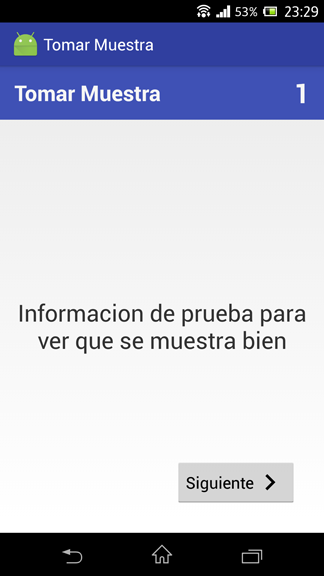
\includegraphics[scale=0.4]{05-implementacion/InformationStep.png} 
   \caption{Ejemplo de un InformationStep en ejecución}
   \label{fig:imgInformationStep}
\end{figure}

\subsubsection{InformationStepResult: El resultado de Mostrar información}
El resultado de mostrar información es nulo, es una clase vacía. Solo está para cerrar el circuito.

\subsection{PhotoStep: Tomar una foto}
PhotoStep se usa para solicitarle al científico ciudadano que tome una foto. Tiene un texto (instructionsToShow) que se muestran a modo de instrucciones o mensaje cuando la cámara esta encendida. Luego de tomada la foto, se muestra una vista preliminar de la misma, con un botón que da la opción de volver a tomar la foto.

En Android Studio (Java):
\begin{lstlisting}[language=Java, frame=tlb]	
PhotoStep step = new PhotoStep(1,"Por favor tome una foto de su gato",2);
\end{lstlisting}

Usando el generador de clases:
\begin{lstlisting}[language=XML, frame=tlb]	
{
  "id" : 1,
  "type" : "Photo",
  "text" : "Por favor tome una foto de su gato",
  "nextStepId" : 2
}
\end{lstlisting}

\begin{figure}[H]
  \centering
    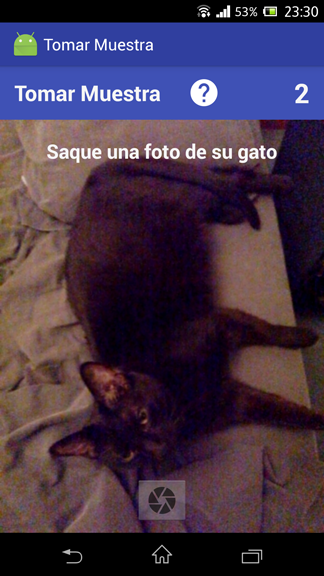
\includegraphics[scale=0.4]{05-implementacion/PhotoStep1.png} 
    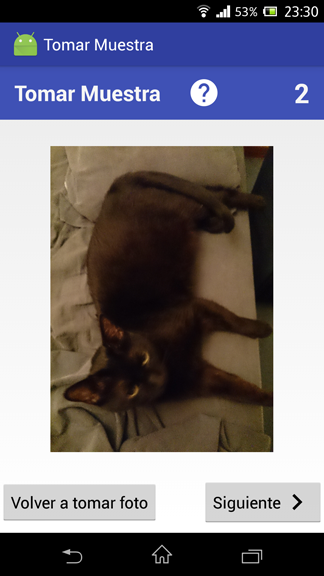
\includegraphics[scale=0.4]{05-implementacion/PhotoStep2.png}     
   \caption{Ejemplo de un PhotoStep en ejecución. A la izquierda al momento de tomar la foto, y a la derecha al momento de mostrar la vista preliminar.}
   \label{fig:imgPhotoStep}
\end{figure}

\subsubsection{PhotoStepResult: El resultado de Tomar una foto}
guarda el imageFileName de la foto. 
La foto va como archivo jpg en la carpeta de la muestra.
Puede haber varias fotos si hay varios PhotoSteps en el workflow

\subsection{SoundRecordStep: Grabar sonido}
Tiene instructionsToShow a modo de instrucciones que se muestran.

En Android Studio (Java):
\begin{lstlisting}[language=Java, frame=tlb]	
SoundRecordStep step = new SoundRecordStep(1,"Grabe el sonido de su auto",2); 
\end{lstlisting}

Usando el generador de clases:
\begin{lstlisting}[language=XML, frame=tlb]	
{
  "id" : 1,
  "type" : "Sound",
  "text" : "Grabe el sonido de su auto",
  "nextStepId" : 2
}
\end{lstlisting}

\subsubsection{SoundRecordStepResult: El resultado de Grabar sonido}
guarda el soundFileName del sonido.
El sonido va como archivo mp4 en la carpeta de la muestra.
Puede haber varios sonidos si hay varios SoundRecordSteps en el workflow


\subsection{SelectOneStep: Seleccionar una opción de un grupo de opciones}
Tiene un title
Las opciones son una lista de objetos SelectOneOption
Cada objeto SelectOneOption tiene un id, textToShow y nextStepId
Explicar la bifurcación de caminos en el workflow a partir de este Step
En forma de radio buttons

En Android Studio (Java):
\begin{lstlisting}[language=Java, frame=tlb]	
ArrayList<SelectOneOption> optionsToSelectOne = new ArrayList<SelectOneOption>();
optionsToSelectOne.add(new SelectOneOption(1,"Opcion 1", 2));
optionsToSelectOne.add(new SelectOneOption(2,"Opcion 2", 2));
optionsToSelectOne.add(new SelectOneOption(3,"Opcion 3", 3));
SelectOneStep step = new SelectOneStep(1,optionsToSelectOne,"Seleccione una opcion");

\end{lstlisting}

Usando el generador de clases:
\begin{lstlisting}[language=XML, frame=tlb]	
{
  "id" : 1,
  "type" : "SelectOne",
  "title" : "Seleccione una opcion",
  "options" : [
    {
      "id":1,
      "text":"Opcion 1",
      "nextStepId" : 2
    },
    {
      "id":2,
      "text":"Opcion 2",
      "nextStepId" : 2
    },
    {
      "id":3,
      "text":"Opcion 3",
      "nextStepId" : 3
    }
  ]
}
\end{lstlisting}

\subsubsection{SelectOneStepResult: El resultado de Seleccionar una opción de un grupo de opciones}
El resultado tiene la opción seleccionada (un objeto SelectOneOption)

\subsection{MultipleSelectStep: Seleccionar varias opciones de un grupo de opciones}
Tiene un title
Las opciones son una lista de objetos MultipleSelectOption
Cada objeto MultipleSelectOption tiene un id y textToShow
en forma de checkboxes

En Android Studio (Java):
\begin{lstlisting}[language=Java, frame=tlb]	
ArrayList<MultipleSelectOption> optionsToSelect = new ArrayList<MultipleSelectOption>();
optionsToSelect.add(new MultipleSelectOption(1,"Arboles"));
optionsToSelect.add(new MultipleSelectOption(2,"Basura"));
optionsToSelect.add(new MultipleSelectOption(3,"Agua"));
optionsToSelect.add(new MultipleSelectOption(4,"Animales"));
MultipleSelectStep step = new MultipleSelectStep(1,optionsToSelect,"Seleccione lo que ve",2); 
\end{lstlisting}

Usando el generador de clases:
\begin{lstlisting}[language=XML, frame=tlb]	
{
  "id" : 1,
  "type" : "MultipleSelect",
  "title" : "Seleccione lo que ve",
  "options" : [
    {
      "id":1,
      "text":"Arboles"
    },
    {
      "id":2,
      "text":"Basura"
    },
    {
      "id":3,
      "text":"Agua"
    },
    {
      "id":4,
      "text":"Animales"
    }
  ],
  "nextStepId" : 2
}
\end{lstlisting}

\subsubsection{MultipleSelectStepResult: El resultado de Seleccionar varias opciones de un grupo de opciones}
El resultado tiene una lista de las opciones seleccionadas (una lista de objetos MultipleSelectOption)



\subsection{LocationStep: Posicionar la muestra en el mapa con el GPS}
Tiene un textToShow a modo de instrucciones
Permite usar el GPS o posicionar la muestra manualmente en el mapa

En Android Studio (Java):
\begin{lstlisting}[language=Java, frame=tlb]	
LocationStep step = new LocationStep(1,"Por favor posicione la muestra en el mapa",2); 
\end{lstlisting}

Usando el generador de clases:
\begin{lstlisting}[language=XML, frame=tlb]	
{
  "id" : 1,
  "type" : "Location",
  "text" : "Por favor posicione la muestra en el mapa",
  "nextStepId" : 2
}
\end{lstlisting}

\subsubsection{LocationStepResult: El resultado de Posicionar la muestra en el mapa con el GPS}
Guarda latitude y longitude

\subsection{RouteStep: Grabar un recorrido en el mapa usando el GPS}
Tiene un textToShow a modo de instrucciones
Intervalo y mapZoom opcionales. Poner los valores por defecto

En Android Studio (Java):
\begin{lstlisting}[language=Java, frame=tlb]	
RouteStep step = new RouteStep(1,"Registre la ruta que corre",2); 
step.setInterval(10000);
step.setMapZoom(18);
\end{lstlisting}

Usando el generador de clases:
\begin{lstlisting}[language=XML, frame=tlb]	
{
  "id" : 1,
  "type" : "Route",
  "text" : "Registre la ruta que corre",
  "interval" : 10000,
  "mapZoom" : 18,
  "nextStepId" : 2
}
\end{lstlisting}

\subsubsection{RouteStepResult: El resultado de Grabar un recorrido en el mapa usando el GPS}
guarda una lista de objetos Location

\subsection{InsertTextStep: Ingresar texto}
textToShow a modo de instrucciones
sampleText a modo de ejmplo
maxLength cantidad máxima de caracteres permitida
Type Values allowed are: text, number or decimal
optional indicando si se puede dejar vacío y no ingresar ningún texto (true) o si se requiere que ingrese algo si o si (false)


En Android Studio (Java):
\begin{lstlisting}[language=Java, frame=tlb]	
InsertTextStep step = new InsertTextStep(1,"Por favor, ingrese el nombre del lago","Nombre del lago",50,InsertTextStep.InputType.TYPE_TEXT,true,2);
\end{lstlisting}

Usando el generador de clases:
\begin{lstlisting}[language=XML, frame=tlb]	
{
  "id" : 1,
  "type" : "InsertText",
  "text" : "Por favor, ingrese el nombre del lago",
  "sampleText" : "Nombre del lago",
  "inputType" : "text",
  "maxLength" : 50,
  "optional" : true,
  "nextStepId" : 2
}
\end{lstlisting}

\subsubsection{InsertTextStepResult: El resultado de Ingresar texto}
guarda el texto ingresado en insertedText

\subsection{InsertDateStep y InsertTimeStep: Ingresar fecha y hora}
ambos tienen textToShow a modo de instrucciones

En Android Studio (Java):
\begin{lstlisting}[language=Java, frame=tlb]	
InsertDateStep step = new InsertDateStep(1,"Por favor indique la fecha de la muestra",2); 
\end{lstlisting}

Usando el generador de clases:
\begin{lstlisting}[language=XML, frame=tlb]	
{
  "id" : 1,
  "type" : "InsertDate",
  "text" : "Por favor indique la fecha de la muestra",
  "nextStepId" : 2
}
\end{lstlisting}

En Android Studio (Java):
\begin{lstlisting}[language=Java, frame=tlb]	
InsertTimeStep step6 = new InsertTimeStep(1,"Por favor indique la hora de la muestra",2); 
\end{lstlisting}

Usando el generador de clases:
\begin{lstlisting}[language=XML, frame=tlb]	
{
  "id" : 1,
  "type" : "InsertTime",
  "text" : "Por favor indique la hora de la muestra",
  "nextStepId" : 2
}
\end{lstlisting}

\subsubsection{InsertDateStepResult y InsertTimeStep: El resultado de Ingresar fecha y hora}
un objeto Date que tiene la fecha o la hora según corresponda

\section{Mostrar Ayuda}

\section{Usando autenticación} \label{sec:usando_autenticacion}
Por defecto provee autenticación con Google, porque al tener Android tiene una cuenta de Google si o si.
Esta abierto a poder agregar autenticación con otras plataformas/APIs.

Samplers provee autenticación con Google, pero ese necesario registrar la aplicación en la pagina de desarrolladores de google (https://developers.google.com/identity/sign-in/android/start-integrating). Ahí hay que seguir los pasos para [to Configure a Google API Console project]. Es necesario [proveer] el nombre de la aplicación, package name, y también el SHA-1 hash del certificado con el que se firma la aplicación.

Una vez registrada la aplicación en Google, hay que configurar Samplers para habilitar la autenticación.

Una vez configurado los valores de los parámetros de autenticación, Samplers mostrará un fragment de inicio de sesión la primera vez que el usuario intente tomar una muestra. Si la autentición es opcional, se mostrará un botón para omitir el inicio de sesión y continuar con la toma de la muestra. También se muestra un botón para iniciar sesión en la activity principal (si se está usando la que provee Samplers).

Cuando la muestra es enviada, el id de usuario y el método de autenticación (por defecto 'google') se envían junto con esta.


\subsection{Configurar autenticación con el generador de clases de Gradle}

Para usar autenticación usando el generador de clases de Gradle, es necesario configurar los siguientes parámetros en el objeto \textbf{applicaction}:

\begin{itemize}

	\item \textbf{authenticationEnabled}: poner en true para habilitar la autenticación
		
	\item \textbf{authenticationOptional}: poner en true si se desea que la autenticación sea opcional, o en false si se desea que la autenticación sea obligatoria.
	
	\item Dentro del parámetro \textbf{networkConfiguration} es necesario establecer los parámetros \textbf{paramNameUserId} y \textbf{paramNameAuthenticationType} con los nombres de los parámetros con los que irán el id de usuario y el tipo de autenticación usada respectivamente dentro del mensaje HTTP POST.
	

\end{itemize}

Ejemplo:

\begin{lstlisting}[language=XML, frame=tlb]	
{
  "application": {
    "title" : "Samplers Hello World App",
    "welcomeMessage" : "Welcome to your first Samplers App!",
    "networkConfiguration" : {
      "url" : "http://192.168.1.10/samplers/upload.php",
      "paramName" : "sample",
      "paramNameUserId" : "user_id",
      "paramNameAuthenticationType" : "authentication_type"
    },
    "authenticationEnabled" : true,
    "authenticationOptional" : true
  } 
}
\end{lstlisting}

\subsection{Configurar autenticación [con instanciación manual]}

Para usar autenticación [con instanciación manual], es necesario definir la configuración de red y de autenticación en el método \textbf{onCreate()} de la activity principal:

\begin{lstlisting}[language=Java, frame=tlb]	
@Override
protected void onCreate(Bundle savedInstanceState) {
  super.onCreate(savedInstanceState);
	
  NetworkConfiguration.setURL("http://192.168.1.10/samplers/upload.php");
  NetworkConfiguration.setPARAM_NAME_SAMPLE("sample");
  // Set the authentication params of the Network Configuration
  NetworkConfiguration.setPARAM_NAME_USER_ID("user_id");
  NetworkConfiguration.setPARAM_NAME_AUTHENTICATION_TYPE("authentication_type");

  // Set the authenticationconfiguration
  AuthenticationManager.setAuthenticationEnabled(true);
  AuthenticationManager.setAuthenticationOptional(true);
}
\end{lstlisting}

\subsection{Usando un método de autenticación propio} \label{sec:usar_auth_propia}

Con Samplers también se puede usar un método de autenticación propio, definiendo un LoginFragment y una clase User (o varias clases si se desea proporcionar autenticación con diferentes APIs, como Facebook, Tweeter, Yahoo, etc.) y Samplers enviará junto con la muestra el id de usuario y el método de autenticación usado.


\subsubsection{Definiendo un Login Fragment [personalizado]}

Es necesario crear un fragment que herede de LoginFragment, y configurar la clase AuthenticationManager para que lo use, llamando al método setLoginFragmentClass() dentro del método onCreate() de la ativity principal:

\begin{lstlisting}[language=Java, frame=tlb]	
@Override
protected void onCreate(Bundle savedInstanceState) {
  super.onCreate(savedInstanceState);
	
  AuthenticationManager.setLoginFragmentClass(MyCustomLoginFragment.class);
}
\end{lstlisting}

El proceso de login y la interacción con las APIs responsabilidad del desarrollador, pero después de que el usuario inicia sesión en la API seleccionada, es necesario llamar al método login() en la clase AuthenticationManager y al método onLogin() en el objeto mListener heredado:

\begin{lstlisting}[language=Java, frame=tlb]	
if (loginOK) {
  AuthenticationManager.login(user, getActivity().getApplicationContext());
  mListener.onLogin(user);
}
\end{lstlisting}


\subsubsection{Definiendo una clase User [personalizada]}

Es necesario crear una clase usuario propia que implemente la interfaz User por cada método de autenticación que se use. Los objetos de dichas clases se usarán para llamar al método login() de la clase AuthenticationManager.

Ejemplo de una clase usuario propia:
\begin{lstlisting}[language=Java, frame=tlb]	
public class EMailUser implements User {

    public static final String AUTHENTICATION_TYPE = "email";

    private String userName;
    private String email;

    public GoogleUser(String userName, String email) {
        this.userName = userName;
        this.email = email;
    }

    @Override
    public String getAuthenticationType() {
        return AUTHENTICATION_TYPE;
    }

    @Override
    public String getUserName() {
        return userName;
    }

    @Override
    public String getUserId() {
        return email;
    }

}
\end{lstlisting}



\section{Personalización}

\subsection{Temas y colores}

\subsection{Idiomas}

\section{Definir un nuevo Step, StepFragment y StepResult ??} \label{sec:definir_steps}



\chapter{Instanciación del framework: Caso de uso}

\section{AppEar}
[ver si esto lo ponemos o no, porque no sabemos como quedó este proyecto al final... Otra alternativa acá sería plantear una app de ejemplo (teórica o una concreta que ya exista) y mostrar como se configuraría en Samplers y poner las capturas de pantalla de la app generada por Samplers]

\section{AppEar usando Samplers}

\section{Comparación y conclusión}
[breve comparacion y conclusion]
\chapter{Conclusiones y Trabajo Futuro}

[falta desarrollar...]

%Supongamos que se quiso atacar el problema de la dificultad en el desarrollo de aplicaciones móviles multi-plataforma. Y que lo que se hizo fue desarrollar una librería de clases. ¿Cómo demuestro que la librería de clases resuelve el problema?

%Antes que nada, deberíamos haber dejado claro, en alguna sección del capítulo \ref{introduccion} cuales son los indicadores que miro para decir que hay "dificultad en el desarrollo de aplicaciones móviles". Por ejemplo, ¿cantidad de bugs específicos de la plataforma? ¿tiempo que lleva traducir los aspectos específicos?. Conocer esos indicadores (o aspectos) es importante para decidir a cuales de ellos voy a apuntar en mi solución (porque tal vez no puedo ser mejor en todos los aspectos). Es importante para poder comparar mi solución con otras. Y es importante porque en este capítulo tengo que demostrar que mi solución es mejor en términos del/los aspectos elegidos. 

%La evaluación se puede hacer de muchas formas y depende del caso en particular. Por ejemplo, podrías poner a varios compañeros a hacer la misma aplicación demo con tu librería y otras que ellos quieran. Y luego les hacés preguntas para saber si con tu libreria fué mejor. O podés contar la cantidad de bugs que se hicieron usando tu librería vs los que se hicieron sin ella. Hacer un experimento es complejo, pero hay muchas alternativas intermedias para que puedas demostrar que tu propuesta resuelve el problema planteado.








%Los artículos que se citan en la tesis, se incluyen en el archivo bibliografía.bib, en formato bibtex.
%En la sección bibliografía, van a aparecer automáticamente aquellos que se citan desde el texto 
%utilizando el comando \cite con la etiqueta correspondiente - en la introducción hay un par de ejemplos. 

\bibliographystyle{ieeetr}
\bibliography{90-bibliografia}


\end{document}
\end

